\documentclass[%
  a4paper,     % Paper size (a5paper)
  10pt,        % Font size  (9,10,11,12)
  twoside,     % two sided printing (oneside)
  openright,   % each chapter starts on rectopage (openleft)
  final,       % useful markings -- change to final when done
               %                    (or ms for a laugh)
]{memoir}

%
% any packages we may need to load
%
% Bibliography packages:
% ---------------------
% We use natbib, as it is neatest
\usepackage[%
  round,          % round brackets
  comma,          % separate multiple citations with comma
  authoryear      % author and year citations
]{natbib}
% Include the references in the title
%\usepackage[nottoc]{tocbibind}
% Use the ADS macros for bibtex
\usepackage{other/aas_macros}


% Graphics packages:
% -----------------
%
% This is for using
%  \includegraphics
%  \graphicspath
%
\usepackage{graphicx}
%
% Colors:
\usepackage{xcolor}


% Hyperlink packages:
% ------------------
\usepackage[             % hyperlinks 
  colorlinks=true,       %  -- set so only external links
  urlcolor={blue},       %     are highlighted
  linkcolor={black},
  citecolor={black},
  pdfborder={0 0 0}
]{hyperref}



% Quotes:
% ------
\usepackage{epigraph}


% TiKz:
% -----
\usepackage{tikz}     % The tikz package
\usepackage{pgfplots} % For plotting functions

% Tikz libraries:
% ---------------
%\usetikzlibrary{<++>}





% Table of contents:
% -----------------
%
% This enables a shorter table of contents
\usepackage{shorttoc}

% Word count package:
% ------------------



% Maths
\usepackage{amsmath} % AMS styles (align etc)
\usepackage{amssymb} % ----------''----------

\usepackage{upgreek} % upright greek symbols


% For draft text
\usepackage{ifdraft}



%
% any commands that should be defined
\newcommand{\people}[2]{\href{#1}{\color{black}{#2}}}

\newcommand{\davidmackay}{%
  \people{%
    http://www.inference.phy.cam.ac.uk/mackay/%
  }{%
    David MacKay%
  }%
}

\newcommand{\rafiblumenfeld}{%
  \people{%
    http://www.imperial.ac.uk/people/r.blumenfeld%
  }{%
    Rafi Blumenfeld%
  }%
}

\newcommand{\stevegull}{%
  \people{%
    http://www.phy.cam.ac.uk/directory/gulls%
  }{%
    Steve Gull%
  }%
}

\newcommand{\edjaynes}{%
  \people{%
    https://en.wikipedia.org/wiki/Edwin_Thompson_Jaynes%
  }{%
    Ed Jaynes%
  }%
}

\newcommand{\johnskilling}{%
  \people{%
    http://www.maxent.co.uk/john.html%
  }{%
    John Skilling%
  }%
}
    %References to people
\input{commands/programs}  %code commands
% command to count words in document
\newcommand\wordcount{
%  \immediate\write18{texcount -inc -sum=1,1,1,1,1,1,1 -0 -template={SUM} thesis.tex 2> /dev/null | sed '/^$/d' > other/count.txt}
  \input{other/count.txt} }
     %tex tools

% Probabilities
\newcommand{\Probc}[2]{\mathrm{P}\left(#1\middle|#2\right)}
\newcommand{\Prob}[1]{\mathrm{P}\left(#1\right)}

\newcommand{\posterior}{\mathcal{P}}   % Posterior
\newcommand{\lik}{\mathcal{L}}         % Likelihood
\newcommand{\prior}{\pi}               % Prior
\newcommand{\ev}{\mathcal{Z}}          % evidence
\newcommand{\data}{\mathcal{D}}        % Data
\newcommand{\params}{\theta}           % parameters
\newcommand{\model}{\mathcal{M}}       % Model


  %Bayesian nomenclature
% define the font for programs
\newcommand{\programscript}[1]{{\textsc #1}}              % Font for progs


% Ineference codes
\newcommand{\PolyChord} {\programscript{PolyChord}}     % PolyChord
\newcommand{\MultiNest} {\programscript{MultiNest}}     % MultiNest

% Programming languages
\newcommand{\FORTRAN}   {\programscript{FORTRAN}95}       % FORTRAN
\newcommand{\Cpp}       {\programscript{C++}}                 % C++    
\newcommand{\openMPI}   {\programscript{openMPI}}         % openMPI

% Cosmology codes
\newcommand{\CosmoMC}   {\programscript{CosmoMC}}         % CosmoMC
\newcommand{\CAMB}      {\programscript{CAMB}}               % CAMB
\newcommand{\CosmoChord}{\programscript{CosmoChord}}   % CosmoChord
\newcommand{\ModeCode}  {\programscript{ModeCode}}       % ModeCode
\newcommand{\ModeChord} {\programscript{ModeChord}}     % ModeChord
      %code
%   possessive citation
\newcommand{\citepos}[1]{\citeauthor{#1}'s (\citeyear{#1})}
    %bibliographic
\newcommand{\prm}[1]{{{#1}^\prime}}           % #1^\prime 
\newcommand{\dprm}[1]{{{#1}^{\prime\prime}}}  % #1^{\prime\prime}


% Math operators
\DeclareMathOperator{\sech}{sech}
\DeclareMathOperator{\csch}{csch}
\DeclareMathOperator{\arcsec}{arcsec}
\DeclareMathOperator{\arccot}{arccot}
\DeclareMathOperator{\arccsc}{arccsc}
\DeclareMathOperator{\arccosh}{arccosh}
\DeclareMathOperator{\arcsinh}{arcsinh}
\DeclareMathOperator{\arctanh}{arctanh}
\DeclareMathOperator{\arcsech}{arcsech}
\DeclareMathOperator{\arccsch}{arcCsch}
\DeclareMathOperator{\arccoth}{arcCoth} 
     %maths
\newcommand{\meff}{m_\mathrm{eff}}
\newcommand{\meffs}{m_\mathrm{eff}^2}
 %constants
%


\includeonly{%
other/thanks,
chapter_bayesian_inference/bayesian_inference
}

\begin{document}
%
% title page
%
\title{Kinetic initial conditions for inflation:\\ {\large Theory, observations and methods}}

\author{Will Handley\\
Cavendish Astrophysics \\
Gonville \& Caius}
\date{Due to be submitted: March 2016}

\maketitle

\centerline{%
 A dissertation for the degree of Doctor of Philosophy
in the University of Cambridge }


%
% contents ...
%

% Display a short table of contents

\setcounter{tocdepth}{0}
\renewcommand*\contentsname{Contents}
\tableofcontents*
\cleardoublepage{}
% Now display a longer table of contents
\setcounter{tocdepth}{1}
\renewcommand*\contentsname{Contents (detailed)}
\tableofcontents*

\cleardoublepage{}

%
% summary ...
%
\chapter*{Summary}

\addcontentsline{toc}{chapter}{Summary}

This is the summary.
%
Here is a url: \url{http://www.mrao.cam.ac.uk/~dag/}



%
% declaration ...
%
\chapter*{Declaration}

\addcontentsline{toc}{chapter}{Declaration}

Word Count: \wordcount{}words (including text, headers, captions, floats, inlined formulae and displayed formulae).


This is the declaration. This is not too long, honest!

\cleardoublepage{}

%
% thanks ...
%
\chapter*{Acknowledgements}

\addcontentsline{toc}{chapter}{Acknowledgements}

To Professors Anthony Lasenby and Mike Hobson. One could not hope for more supportive and caring supervisors. I can only hope that one day I will be able to pass the favour to the next generation of students with half as much skill and grace.

Thanks are due to all of my teachers over the past twenty-six years. Special mention goes to my Mathematics and Science teachers at Alleyn's School: Ed Mann, Anne Poole, Neil Kinner, Sara Hopley and Margaret Hunnibal. At Cambridge I must thank Rafi Blumenfeld, Derek Barnes, Adam Thorne, David Summers, Ulrich Kaiser, Steve Gull, Paul Alexander \& John Ellis. Having experienced supervising from both sides now, I know how difficult a student I must have been.

I am very grateful to have the support and care of the astrophysics administrator Karen Scrivener. 

To my office mates Sonke Hee, Richard Wolstenhulme and Do Young,

To my mother and father for all of their love and support over the years.

Last and most to my fianc\'{e}e

%Many thanks are due to the moderators and posters on the \mbox{\href{http://stackexchange.com/}{StackExchange}} forums. You are the unsung heroes and heroines of the modern internet age.
%
%\begin{itemize}
%  \item Mike and Anthony
%  \item All teachers (brief). 
%  \item Karen Scrivener
%  \item Office mates
%  \item Mum and Dad
%  \item Sophie (last and most)
%\end{itemize}

\cleardoublepage{}

%
% chapters ...
%
% Outline
% -------
%
\graphicspath{{.}{./chapter_outline/figures/}}
\chapter{Outline}
\label{chap:out}

\section{The big picture}
\begin{figure}[tp]
  \includegraphics[width=\textwidth]{chapter_outline/figures/planck}
  \caption{Planck's image of the early universe}\label{fig:out:planck}
\end{figure}

As cosmologists, nature has been incredibly kind to us. We have been given a near crystal clear snapshot of the universe a mere 300,000 years after its birth. Images taken by the Planck satellite (Figure~\ref{fig:out:planck}) show the universe at this time, detailing the regions of higher and lower density. For cosmologists this is interesting in two ways. 

First, these distortions in density are the beginnings of the formation of stars, galaxies and galaxy clusters. If one were to wind the clock forwards from this moment, cosmic structure would be seen coalescing around the regions of higher density.

Second, these distortions tell us a great deal about physics at much earlier times. Observations from particle physics experiments allow us to confidently wind the clock backwards to mere microseconds after the big bang.
However, the expansion of the universe itself allows us to look even further back than this. We now have a wealth of observational evidence that early in its history, the universe went though a rapid accelerated epoch.  This expansion acts as a cosmic magnifying glass, allowing us to observe patterns $\sim10^{-32}$ seconds after the big bang using the universe we see today. The upshot of this is that cosmologists effectively have access the to most powerful particle accelerator imaginable, trillions of times stronger than the Large Hadron Collider. 

The canonical explanation for the early period of accelerated expansion is the theory of inflation, with quantum fields providing the necessary driving force. This thesis focusses on the initial conditions for inflation; i.e.\ what started this all off.

\section{Kinetic initial conditions}

Traditionally, cosmologists work under the assumption that at these early times the universe was in an effectively eternal inflating state, with no detectable beginning. Chapter~\ref{chap:kd} rigorously proves a result that suggests this picture may be somewhat incomplete. In fact, almost all classical universes begin at a finite time in the past. Moreover, this beginning is dominated by kinetic energy, and not inflating. This provides a novel and arguably simpler mechanism for setting the initial conditions of the universe. More importantly, I also show that this period could have produced a distinct observational signature in the primordial power spectrum of curvature perturbations.

In an attempt to search for evidence of this signal, I became a member of the Planck collaboration. Chapter~\ref{chap:rec} details a model-independent reconstruction of the primordial spectrum. Whilst not conclusive, it did show tantalising hints of a signal consistent with a pre-inflationary epoch.

\section{Observations in high dimensions}
\begin{figure}[tp]
  \includegraphics[width=\textwidth]{chapter_outline/figures/planck_galaxy}
  \caption{The actual image taken by Planck}\label{fig:out:planck_galaxy}
\end{figure}
Planck's view of the early universe is not in fact the one shown in Figure~\ref{fig:out:planck}. The picture it actually takes is more akin to Figure~\ref{fig:out:planck_galaxy}. The most notable difference between the two is the presence of a red band in the center of the image, which are the microwaves emitted by our own Milky Way galaxy. In order to observe the microwaves generated by the beginning of the universe, we must first remove the contaminating information of the Milky Way. This requires a sophisticated model of the galaxy, with many parameters that must be simultaneously determined and quantified. 

Whilst working on Planck, it became apparent that the principle difficulty of searching for this signal was an absence of data analysis tools. There was no serviceable method for analysing complicated Bayesian models such as those found in the galactic foregrounds.

The Cavendish astrophysics department has a long history of proposing and developing novel Bayesian statistical approaches. With this in mind, I designed and implemented a novel algorithm which was christened PolyChord (detailed in Chapter~\ref{chap:pc}). This was designed to gather information from data about complicated scientific models, whilst simultaneously calculating the probability that the model is true. PolyChord proved extremely successful in the Planck analysis, and was rapidly adopted by many members of the team as its de-facto inference tool

\section{Quantum initial conditions}
My latest work focusses on the quantum mechanical initial conditions of the early universe. A full theoretical treatment of this epoch requires a consideration of quantum fields in curved spacetime. One of the critical issues is that our basic ideas about how we talk about quantum particles are not designed to work in the context of gravity as a curved spacetime background. My latest research aims to resolve some of these issues, by re-defining the quantum mechanical notion of empty space, and building a vacuum around the renormalised stress energy tensor. I also demonstrated that in the context of the early universe this alternative viewpoint makes detectable predictions which again differ from standard theory. This is detailed in Chapter~\ref{chap:qv}.

Whilst examining this, I realised that I needed a better way of solving the equations of the early universe. I did indeed succeed in developing a novel class of extremely efficient numerical methods for solving these, which I term RKWKB approaches. RKWKB is explained Chapter~\ref{chap:RK}.

\section{Thesis versus research}

The theme of this thesis is the interplay between theory, observations and methods. Whilst this book is divided into two parts, in reality both halves have strongly influenced each other in a manner not necessarily consistent with the sequence of the text. Figure~\ref{fig:out:sequence} shows an approximate set of interactions between the various chapters. Whilst a thesis must be laid out sequentially, the reality is that research in the real-world is very non-linear.

\begin{figure}[tp]
  \tikzsetnextfilename{sequence}
  \begin{tikzpicture}[%
    node distance = 5mm,
    writing/.style={%
      text width=25mm,  % default text width
      align=center      % align in center
    },
    component/.style={%
      writing,          % writing style above
    },
    connection/.style={%
      very thick,      % very thick arrows
      >=stealth        % pretty arrow head
    }
]

  \node[component] (KD) at (0,0) {Kinetic dominance\\(Chapter~\ref{chap:kd})};

  \node[above right = of KD, component] (TO)  {Theoretical observations\\(Chapter~\ref{chap:cls})};

  \node[below right = of KD, component] (PS) {Power spectrum reconstruction\\(Chapter~\ref{chap:rec})};

  \node[below left = of PS, component] (NS) {Nested sampling\\(Chapter~\ref{chap:ens})};

  \node[below = of PS, component] (PC) {\PolyChord{}\\(Chapter~\ref{chap:pc})};

  \node[right = of TO, component] (RE) {Quantum\\ kinetic dominance\\(Chapter~\ref{chap:qv})};

  \node[below right = of RE, component] (RK) {RKWKB\\(Chapter~\ref{chap:RK})};

  \node[below left = of RK, component] (FUT) {Future research: constraining the kinetically dominated universe\\(Chapter~$N$)};

    \draw[connection,->] (KD) -- (PS);
    \draw[connection,->] (KD) -- (TO);
    \draw[connection,->] (PS) -- (NS);
    \draw[connection,->] (NS) -- (PC);
    \draw[connection,->] (PC) -- (PS);
    \draw[connection,->] (TO) -- (RE);
    \draw[connection,->] (PS) -- (RE);
    \draw[connection,->] (RE) -- (RK);
    \draw[connection,->] (RE) -- (FUT);
    \draw[connection,->] (PC) -- (FUT);
    \draw[connection,->] (RK) -- (FUT);
    \draw[connection,->] (PS) -- (FUT);

\end{tikzpicture}

  %\includegraphics[width=\textwidth]{chapter_outline/plots/sequence.tikz}
  \caption{The ``sequence'' of my research.}\label{fig:out:sequence}
\end{figure}




%\cleardoublepage{}

%
%
%
%
%
%
% Statistics
% ==========
%
\part{Statistics}
\label{part:statistics}
%
% Bayesian inference
% ------------------
%


\makeatletter
\def\input@path{{.}{./chapter_bayesian_inference/}}
\makeatother
\chapter{Bayesian Inference}
\label{chap:bay}
%\includegraphics[width=\textwidth]{bayesian_evol}

\epigraph{We anticipate the sun will rise tomorrow, not just because it has always done so far, but because this is predicted by {\em models}, which accord with {\em data}. Any perceived failure of the sun to rise would more likely be a hallucination.}{\davidmackay{}}

%  * BRIEF intro to difference between bayesian and frequentist, and the nature of probability
%      - Continuous vs. Discrete
%      - Aleatoric vs. Epistemological \davidspiegelhalter
%
%  * Parameter estimation and model comparison
%       -Example? (e.g.\ coin flipping, --- anything better?)
%
%  * Sampling as method for describing high-dimensional probability distributions.
%      - MH as good technique
%      - Need for evidences


Science is not the search for truth. Instead, scientists concern themselves with the construction of models. These models have their relative merit determined using data.\footnote{The opening statement of this chapter was in fact the first thing \rafiblumenfeld{} said to us for our part IB Physics supervisions.}

% Mathematics -- if then, conditional truth
% Science -- weaker: observations -> possibilities 

\section{Probability}
\label{sec:bay:prob}

Probability is the mathematical language of uncertainty. It is a methodology of assigning a numerical weighting to outcomes or {\em events}. An event is any subset of the sample space $\Omega$. Some examples of discrete and continuous sample spaces are:
\begin{enumerate}
  \item The outcome of a coin flip $\Omega_1=\{\mathrm{Heads},\mathrm{Tails}\}$.
  \item The measured position of an electron $\Omega_2=\mathbb{R}$.
\end{enumerate}
For example, an event could be that the electrons position $x$ is measured to be $-1<x<0.5$. The role of probability is to assign a weighting to all subsets, which roughly corresponds to the ``chance'' that such an event would occur. Probability should therefore be additive:
\begin{equation}
  A,B \mathrm{\ disjoint} \Rightarrow \Prob{A \cup B} = \Prob{A} + \Prob{B}.
  \label{eqn:bay:add}
\end{equation}
One also normalises the probability distribution so that $\Prob{\Omega} = 1$. The above is effectively a paraphrasing of Kolmogorov's axioms of probability.

%In addition, if one has two disjoint sample spaces, for example $\Omega_1$ and $\Omega_2$ mentioned above, one may combine these into a single samples space ${\Omega=\Omega_1\otimes\Omega_2}$, then probability should be multiplicative.





This entire section may be summarised succinctly and formally as:
\begin{quote}
  Probability is any additive mapping $\mathrm{P}$ from the power set $2^\Omega$ of the sample space $\Omega$ to $[0,1]\in \mathbb{R}$, such that $\Prob{\Omega}=1$.
\end{quote}
\johnskilling{} has derived probability from measurement-theoretical grounds\citep[chap. 1]{Bayesian_methods_in_cosmology}, which provides a more intuitive backing to the definition.




\subsection{Bayes' theorem}


\begin{figure}
  \centerline{%
    \def\firstcircle{(-0.75,0) circle (1.5)}
\def\secondcircle{(0.75,0) circle (1.5)}

\begin{tikzpicture}
  \draw \firstcircle;
  \draw \secondcircle;
  \draw (-3,-2) rectangle (3,2);

  \begin{scope}
    \fill[blue!30!white] \firstcircle;
    \clip \secondcircle;
  \end{scope}

  \begin{scope}
    \clip \firstcircle;
    \fill[blue!60!white] \secondcircle;
  \end{scope}

  \draw[above left] node at (-1,0) {\(A\)};
  \draw[above right] node at (1,0) {\(B\)};
  \draw[below ] node at (0,0) {\(A\cap B\)};
  \draw[below left] node at (3,2) {\(\Omega\)};


\end{tikzpicture}


  }
  \caption{Beer-mat mathematics. This diagram is how \edjaynes{} explained Bayes' theorem to a young \stevegull{}. Out of the entire sample space $\Omega$, if we observe $A$ to be true (blue region), then the probability of $B$ given that we know $A$ is simply $\Prob{A\cap B}/\Prob{A}$. Bayes' theorem then follows by rearrangement and symmetry.}
\end{figure}


From this definition, it is useful to define conditional probability via:
\begin{equation}
  \Probc{B}{A} = \frac{\Prob{A\cap B}}{\Prob{A}}.
  \label{eqn:bay:cond}
\end{equation}
Multiplying both sides by $\Prob{A}$, and noting the symmetrical alternative:
\begin{equation}
  \Probc{B}{A}\Prob{A} = \Prob{A\cap B} = \Probc{A}{B}\Prob{B},
  \label{eqn:bay:sym}
\end{equation}
one may then derive Bayes' theorem:
\begin{align}
  \Probc{B}{A} &= \frac{\Probc{A}{B}\Prob{B}}{\Prob{A}}.\\
  \label{eqn:bay:bayes}
  \tag{Bayes' Theorem}
\end{align}
\section{Bayesian vs.\ Frequentist}
\label{sec:bay:bayesian_frequentist}

Whilst the previous section outlined the properties that probability must satisfy, it has not detailed how one should assign probability. Indeed, we have merely referred to probability as a measure of ``chance'', but declined to define what this means.

There are two fundamental types of probability: {\em Aleatoric\/} and {\em Epistemological}. Aleatoric systems are genuinely random, for example: the flip of a coin, or the click on a Geiger counter. Epistemological probability governs systems where the randomness is associated with a subjective lack of knowledge. For example, before prince George was born, bookmakers took bets on whether William and Kate's baby was a boy or a girl. 

The Frequentist school of thought defines probability as:
\begin{description}
  \item[Frequentist Probability:]``The limiting relative frequency of an event.''
\end{description}
I.e.\ if a coin has $\Prob{\mathrm{Head}}=\frac{1}{2}$, then if you were to toss it an arbitrarily large number of times, the fraction of times one would get closer and closer to $\frac{1}{2}$. This is the version of probability that most people encounter early in their mathematical education, but it has several issues.

This definition applies relatively well to Aleatoric systems (since an experiment can often be run a large number of times). However, for epistemological systems, it is all but useless. The frequentist solution is therefore to disregard the latter kind of probability.

Most people's experiences with probability will likely involve betting scenarios, such as William and Kate's baby. Here it is obvious that the betting odds should be approximately $1:1$,\footnote{Betting odds of $a:b$ against indicates a probability of success of $\frac{b}{a+b}$.}\footnote{In fact the probability of a boy being conceived across the population is roughly 51\%, in order to biologically account for male infant mortality. An individual's probability of conceiving a boy or a girl will vary from person to person and in time.}\footnote{A good bookmaker will obviously take this into account, and give you slightly worse odds in order to ensure their profit.} but it should be also be clear that these odds most certainly do not refer to an event that can be repeated an arbitrarily large number of times.

The alternative definition of probability is {\em Bayesian\/}:
\begin{description}
  \item[Bayesian Probability:] ``A degree of belief that an event will occur.'' 
\end{description}
Note that Bayesian probability is {\em subjective}, it matters who's degree of belief one is considering. Probabilities are assigned only with a given state of knowledge. Effectively, Bayesians place aleatoric and epistemological probability under the same umbrella. 

Pure mathematics deals in relative truth or falsity, i.e.\ given initial assumptions, all statements are assigned to the set $\{F,T\}\equiv\{0,1\}$. Bayesian probability can be thought of as a blurring of this process, namely from initial assumptions, various conclusions are assigned a number from the continuum between $[0,1]$.

\section{An example: biased coins}
For example, assume that you toss a coin $N=20$ times, and observe a dataset of $\data = 16$ heads. Is this enough to cause us to doubt the fairness of the coin?

The standard model $\model_0$ is that a coin toss consists of a binomial trial with probability $\frac{1}{2}$. Elementary probability tells us that the chance of getting this data is:
\begin{equation}
  \Probc{\data}{\model_0}= {^{N}C_\data} {\left( \frac{1}{2} \right)}^{N}  = 4.6\times 10^{-3}.
  \label{eqn:bay:M0}
\end{equation}
Note that as should be expected, the chance of obtaining this exact dataset is small. 

If we allow for the possibility that the coin could be any probability $p$, we can encapsulate this in a second model $\model_1$.
\begin{equation}
  \Probc{\data}{p,\model_1}= {^{N}C_\data}\: {p}^{\data} {\left(1 - p \right)}^{N-\data} 
  \label{eqn:bay:M1}
\end{equation}
This second model is not ideal, since we haven't specified the parameter $p$. If we choose $p=\frac{1}{2}$ we recover $\model_0$. It is tempting to choose $p$ such that the probability of getting the data is maximised. This would be an example of a {\em maximum likelihood\/} approach. In this case, the method indicates\footnote{Proof left as exercise to the reader.} we should choose $p = \frac{\data}{N}$. 

Maximum likelihood has its drawbacks, particularly in the case of a low volume of data. After $N=1$ toss, it seems a little premature to choose either $p=1$ or $p=0$ depending on whether we see a head or a tail. Instead picking a specific value of $p$, one could instead ``spread your bets'' and consider several different values of $p$. The full generalisation of this is to consider a continuum of models, and define an initial probability distribution $\Probc{p}{\model_1}$. These can be interpreted as our initial assumptions on the value of $p$, or our initial degree of belief in its value
A natural assumption is to try and be as unbiased as possible and assume that $p$ is equally likely to take any value in between $0$ and $1$. We therefore have:
\begin{equation}
  \Probc{p}{\model_1}=\left\{
  \begin{array}{lr}
    1 &:0\le p\le1\\
    0 &:\text{otherwise.}\\
  \end{array}
  \right.\label{eqn:bay:prior1}
\end{equation}
With this distribution, we can work out what the overall probability of obtaining the dataset $\data$ is, by marginalising over all values of $p$:
\begin{align}
  \Probc{\data}{\model_1} 
  &= \int \Probc{\data}{p,\model_1}\Probc{p}{\model_1}\: dp \\
  &= \int_0^1 {^{N}C_\data}\: {p}^{\data} {\left(1 - p \right)}^{N-\data}\: dp \\
  &= \frac{1}{n+1} = 4.8\times10^{-2}
  \label{eqn:bay:marg}
\end{align}
This is quite telling, because our initial choice for $\Probc{p}{\model_1}$~(\ref{eqn:bay:prior1}) indicates that we expect all data sets with equal probability (independent of $\data$). This is therefore a ``minimally suspicious'' choice in spread.

We now have two equations~(\ref{eqn:bay:M0})~\&~(\ref{eqn:bay:marg}) which detail the probability of getting the dataset $\data$ given the choice of model. However, what we are really after is the probability of the model, given the dataset $\Probc{\model}{\data}$. To compute this, we use Bayes' theorem
\begin{equation}
  \Probc{\model}{\data} = \frac{\Probc{\data}{\model}\Prob{\model}}{\Prob{\data}}.
  \label{eqn:bay:bay_md}
\end{equation}
In order to complete the calculation, we must assign a probability to each model. A natural choice is to consider $\Prob{\model_0}=\Prob{\model_1}=\frac{1}{2}$. $\Prob{\data}$ is just a normalising constant, computed as:
\begin{equation}
  \Prob{\data} = \sum_i \Probc{\data}{\model_i}\Prob{\model_i}, 
  \label{eqn:bay:norm}
\end{equation}
so we may finally compute
\begin{equation}
  \Probc{\model_0}{\data} = 0.088 \qquad
  \Probc{\model_1}{\data} = 0.922
  \label{eqn:bay:comp}
\end{equation}
In other words, a betting man would put money on $\model_1$ with odds of $10:1$ for. Another way of thinking of this is that $\model_1$ is ten times better at describing the data than $\model_0$.

$\model_1$ can go further however. We may also use Bayes' theorem to compute 
\begin{equation}
  \Probc{p}{\data,\model_1} = \frac{\Probc{\data}{p,\model_1}\Probc{p}{\model_1}}{\Probc{\data}{\model_1}}.
  \label{eqn:bay:bay_p}
\end{equation}
This here gives us the distribution on $p$ {\em given the data}. Namely, how the data should update our ``spread bet''. We already have the ingredients for the above construction from equations~(\ref{eqn:bay:M1}),~(\ref{eqn:bay:prior1}),~\&~(\ref{eqn:bay:marg}), and given the uniform prior, we find our updated bet on $p$ is proportional to $p^\data{(1-p)}^{N-\data}$, a function of $p$. This is a beta distribution, and is indicated in Figure~\ref{fig:bay:beta}.

\begin{figure}
  \centerline{%
    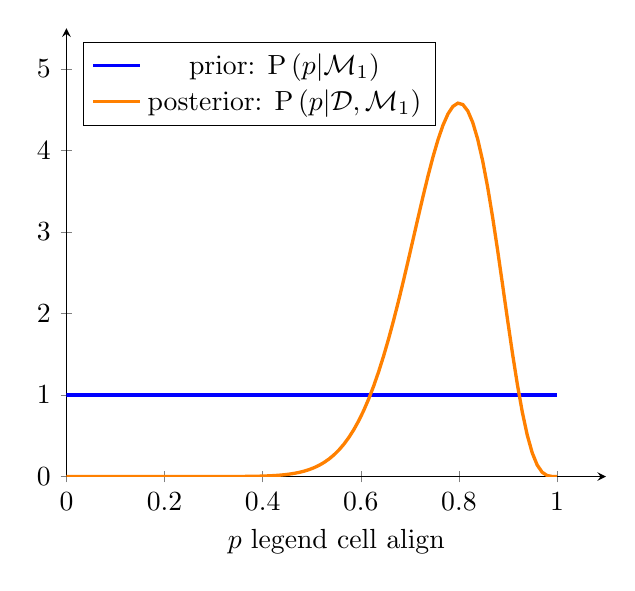
\begin{tikzpicture}[
    declare function={%
      beta(\p,\d,\n)=\p^\d * (1-\p)^(\n-\d) /factorial(\d)/factorial(\n-\d)*factorial(\n+1);
    }
  ]

  \begin{axis}[
      axis lines=left,           % Don't draw box axes
      enlargelimits=upper,       % Extend arrows a little way
      ymax=5,                    % to ensure number 5 is included
      samples=100,               % any fewer and it looks weird
      domain=0:1,                % x range
      xlabel=$p$                 % x label
      legend cell align=left,    % align legend text left
      legend pos= north west,    % put legend in top left
    ]

    \def\pdata{16}    % Number of heads
    \def\pnumber{20}  % Number of coin flips

    % Draw the prior
    \addplot [very thick,blue] {1}; 
    % Add the prior legend
    \addlegendentry{prior: $\Probc{p}{\model_1}$}

    % Draw the posterior
    \addplot [very thick,orange] {beta(x,\pdata,\pnumber)}; 
    % Add the posterior legend
    \addlegendentry{posterior: $\Probc{p}{\data,\model_1}$}

  \end{axis}
\end{tikzpicture}

  }
  \caption{%
  Beta function.\label{fig:bay:beta}
}
\end{figure}

\section{Parameter Estimation \& Model Comparison}
\label{sec:bay:model_comp}
We shall now take the concepts of the previous section, and put them in a general setting. 

The typical problem of science is the construction of a model $\model$ in order to explain some dataset $\data$. Typically, scientific models have a set of continuous parameters $\params_\model$, where $\params_\model$ is normally multi-dimensional, and may contain a variety of parameter types such as integers, vectors, tensors and more exotic components.

Elementary probability theory then enables us to calculate the probability of the data, given the choice of model along with a specific parameter choice.
\begin{equation}
  \lik\equiv\Probc{\data}{\params_\model,\model}.
  \label{eqn:bay:lik_def}
\end{equation}
This distribution is called the {\em likelihood}, which is denoted with a calligraphic~$\lik$ to differentiate between rapidly proliferating conditional probabilities. It is also clearer in many situations to supress explicit data, model and/or parameter-dependence of the likelihood, and instead write:
\begin{equation}
  \Probc{\data}{\params_\model,\model}
  \equiv
  \lik_\model(\params_\model)
  \equiv
  \lik(\params)
  \equiv
  \lik_\model
  \equiv
  \lik.\nonumber
\end{equation}
This is a generic overloading technique which I utilise throughout this thesis.

In order to perform Bayesian inference, another requirement of the model $\model$ is that it must specify an initial degree of knowledge of the parameters:
\begin{equation}
  \prior\equiv\Probc{\params_\model}{\model}.
  \label{eqn:bay:prior_def}
\end{equation}
Since no model occurs in isolation, it is generally not difficult to theoretically produce upper and lower bounds on parameter values. The normal strategy is to choose fairly conservative uniform or Gaussian priors on parameter values. In general, the prior should encapsulate the scale and spread of our current expectation of the parameter value.

Once a prior has been specified, the model $\model$ is complete. The scientific aspect of the problem is complete, and the rest mere statistics. Statistical analysis may be neatly partitioned into two problems: {\em model comparison\/} and {\em parameter estimation}.

\subsection{Model comparison}
It is usually the case in science that there is not a single model available to explain the data. Typically one will have a set of models ${\{\model_1,\model_2,\ldots\}}$, which we wish to scientifically determine the relative merits of given the data $\data$.

We may use the prior to marginalise out all parameter dependence of the each model:
\begin{equation}
  \ev\equiv\Probc{\data}{\model} 
  =
  \int  \Probc{\data}{\params_\model,\model}\Probc{\params_\model}{\model}\:d\params_\model.
  \label{eqn:bay:ev_def}
\end{equation}
This quantity is termed the {\em evidence\/} $\ev$, or {\em marginalised likelihood}, and gives the probability of observing the data $\data$, conditioned on the model $\model$. The quantity we seek however is the probability of each model $\model$ given the data $\data$, which may be obtained using Bayes' theorem:
\begin{equation}
  \Probc{\model_i}{\data} = \frac{\Probc{\data}{\model_i}\Prob{\model_i}}{\Prob{\data}}.
  \label{eqn:bay:bayM}
\end{equation}
In order to utilise this however, we must specify our prior degree of belief in each model
\begin{equation}
  \Prob{\model_i} = \priorM_i
\end{equation}
These may have been obtained from previous analyses, but a non-partisan choice would be too choose the models to be equally weighted. The denominator of~(\ref{eqn:bay:bayM}) is then simply a normalising constant, and the posterior degree of belief in each model may be obtained via:
\begin{equation}
  \Probc{\model_i}{\data} 
  \equiv
  \Wmodel_i
  =
  \frac{\ev_i\priorM_i}{\sum_j \ev_j\priorM_j}.
\end{equation}
These model weights $\Wmodel$ may then be used to determine the ``most probable model''. In some cases there is a clear winner, and the other models may be safely discarded, but the more usual scenario is that there are several competing alternatives. It is for this reason that we prefer the term ``model comparison'' to the more oft-quoted {\em model selection}. Additional datasets may determine a clear winner, but in the mean-time the weights $\Wmodel$ can be used to perform proper inference. 

For example, model often predict a distribution for a common derived parameter $\Probc{y}{\model,\data}$.\footnote{E.g.\ in cosmology, various models of the universe will predict an age or curvature of the cosmos} If the data are not strong enough to distinguish a given model, the correct inference on $y$ is to use a posterior which marginalises over all models:
\begin{equation}
  \Probc{y}{\data} 
  = \sum_i\Probc{y}{\data,\model_i}\Probc{\model_i}{\data}
  = \sum_i\Probc{y}{\data,\model_i}\Wmodel_i.
\end{equation}
This fully Bayesian approach has been historically under-utilised due to the difficulties in numerically computing the evidence.



\subsection{Parameter estimation}
Of equal interest to scientists is to ask what the data tells us about the various parameters.  
Bayes' theorem allows us to invert the conditioning in equation~(\ref{eqn:bay:lik_def}) and find the {\em posterior\/} $\posterior$ by combining the likelihood~(\ref{eqn:bay:lik_def}), prior~(\ref{eqn:bay:prior_def}) and evidence~(\ref{eqn:bay:ev_def}):
%
\begin{equation}
  \posterior\equiv
  \Probc{\params_\model}{\data,\model} = \frac{\Probc{\data}{\params_\model,\model} \Probc{\params_\model}{\model}}{\Probc{\data}{\model}},
  \label{eqn:bay:bayes_theorem}
\end{equation}
%
which is schematically written as:
\begin{align}
  \posterior &= \frac{\lik \times \prior }{\ev }
  \label{eqn:bay:bayes_theorem_abbrv}\\
  \mathrm{Posterior} &= \frac{\mathrm{Likelihood} \times \mathrm{Prior} }{\mathrm{Evidence} }
\end{align}
This describes how our initial knowledge $\prior$ of the parameters updates to $\posterior$ in light of the data $\data$. Note that the evidence $\ev$ features in both model selection and parameter estimation, and its computation is therefore of great significance.







\section{Numerical statistics: Sampling}
\label{sec:bay:samp}
Having discussed the theory of Bayesian statistics, we now turn to the more tricky aspect of actually computing these various inferences. The likelihood~(\ref{eqn:bay:lik_def}) $\lik(\params)$ is a routine, if often challenging, quantity to compute. It is the job of observational scientists to provide this function, and for the purposes of inference we may consider it a ``black box''. In general, $\lik$ will be not be analytical, but instead is a numerical and computationally expensive quantity. Any calculation we perform must aim to minimise the number of times we attempt to evaluate $\lik$. The prior $\prior$ is typically much less expensive to compute and is normally expressed using analytic functions such as a uniform or Gaussian distribution.

Typically, in inference calculation we wish to compute quantities that are marginalised over by the posterior. For example means and variances will typically take the form:
\begin{align}
  \mean{f} 
  &= \int f(\params)\posterior(\params)\:d\params,
  \label{eqn:bay:mean}\\
  &= \int f(\params)\frac{\lik(\params)\prior(\params)}{\ev}\:d\params.
\end{align}
Given a likelihood $\like$ and a prior $\prior$, a naive approach would be to first compute the evidence
\begin{equation}
  \ev = \int \lik(\params) \prior(\params) \: d\params,
  \label{eqn:bay:ev_short}
\end{equation}
and then perform the integral~(\ref{eqn:bay:mean}) using a traditional numerical quadrature procedure. In most cases, this method fails at both steps, due to the fact that the dimensionality of the integration is too high for numerical quadrature to succeed.

To see this issue, consider the integration of a function $g$ along $[0,1]$
\begin{equation}
  \int_0^1 g(x) dx \approx \sum\limits_{i=0}^{n} g(x_i) w_i,
\end{equation}
where ${x_i\in[0,1]}$ are the quadrature points ${w_i\in\mathbb{R}}$ are the quadrature weights. For example, if $x_i = \frac{i}{n}$ and $w_i=\frac{1}{n+1}$ then one obtains the left rectangle rule (Figure~\ref{fig:bay:quadrature}). This calculation therefore requires $\bigO{n}$ calculations of the function In the $d$-dimensional case, then one has the generalisation:
\begin{equation}
  \int_0^1\cdots\int_0^1 g(x_1,\cdots,x_d) dx_1\cdots \: dx_d \approx \sum\limits_{i_1,\cdots,i_d=0}^{n} g(x_{i_1},\cdots,x_{i_d}) w_{i_1,\cdots,i_d},
\end{equation}
This calculation however requires $\bigO{n^d}$ function evaluations. This is an exponential scaling with $d$, and is an example of the {\em curse of dimensionality}. Even for modest number of parameters $\left[ d\bigO{4} \right]$ these kind of integrations require unfeasible amounts of computational time. Worse still, for most likelihoods, the region about which $\lik$ is significantly non-zero is much larger than the prior range\footnote{This should be expected, since the data should update the prior by some amount in each dimension.}. The gridding size $n$ must therefore be taken as reasonably large in order to ensure that enough function evaluations occur at the peak.

\begin{figure}
  \centerline{%
    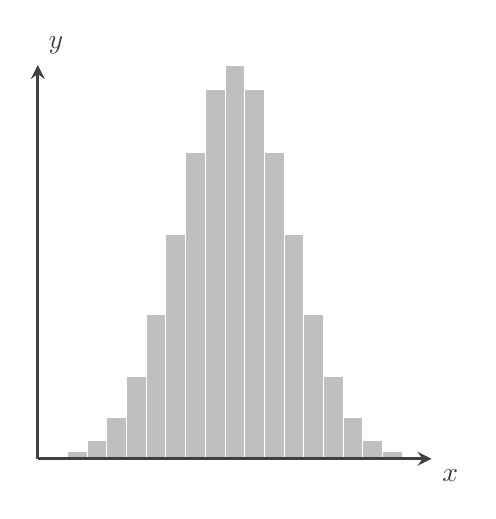
\begin{tikzpicture}[
    declare function={fone(\x)=5*exp(-(\x-2.5)^2);}, 
  very thick, line join=round]

  % Draw squares
  \foreach [evaluate={\x=0.25*\j; \y=fone(\x);}] \j in {0,...,20}{%
    \path [fill=black!25, draw=white, line width=0.2pt] 
    (\x-0.125, 0) -- 
    (\x+0.125, 0) -- 
    (\x+0.125, \y) -- 
    (\x-0.125, \y) -- 
    cycle;
  }

  % Draw functions
%  \draw [black, domain=0.25:4.75, samples=100, variable=\t] 
%  plot (\t, {fone(\t)});

  % x-axis
  \draw [-stealth, black!75] (0,0) -- (5,0) node [below right] {$x$};

  % y-axis
  \draw [-stealth, black!75] (0,0) -- (0,5) node [above right] {$y$};


\end{tikzpicture}

  }
  \caption{\label{fig:bay:quadrature}}
\end{figure}

Fortunately there is a better way. Since we only need points within the region 





\section{Nested Sampling}




%Calculation of the posterior $\posterior(\theta)$ is the domain of {\em parameter estimation}, and in high dimensions is best performed by sampling the space with a Markov-Chain Monte-Carlo approach (MCMC). Examples include Metropolis-Hastings, Gibbs sampling and Slice sampling. For the most part, the evidence $\ev$ is ignored during such calculations, and one works with an unnormalised posterior ${\posterior\propto\lik\times\prior}$.





%
% PolyChord
% ------------------
%
\makeatletter
\def\input@path{{.}{./chapter_polychord/}}
\makeatother
\graphicspath{{.}{./chapter_polychord/figures/}}
\chapter{PolyChord}
\label{chap:pc}

\epigraph{\ldots note that exploring a hard-edged likelihood-constrained domain should prove to be neither more nor less demanding than exploring a likelihood-weighted space }{\johnskilling{}}

\section{Introduction}
\label{sec:pc:introduction}
Over the past two decades, Bayesian methods have been increasingly adopted as the standard inference procedure for the rapidly increasing volume of astrophysical data.

Bayesian inference consists of {\em parameter estimation\/} and {\em model comparison}.  Parameter estimation is generally performed using Markov-Chain Monte-Carlo (MCMC) methods, such as the Metropolis--Hastings (MH) algorithm and its variants~\citep{Mackay}.  In order to perform model comparison, one must calculate the {\em evidence\/}: a high-dimensional integration of the likelihood over the prior density~\citep{Sivia}.  MH methods cannot compute this on a usable timescale, hindering the use of Bayesian model comparison in cosmology and astroparticle physics.

A contemporary methodology for computing evidences and posteriors simultaneously is provided by nested sampling~\citep{skilling2006}. This has been successfully implemented in the now widely adopted algorithm \MultiNest\,~\citep{MultiNest1,MultiNest2,MultiNest3}.  Modern cosmological likelihoods now involve a large number of parameters, with a hierarchy of speeds.  \MultiNest\ struggles with high-dimensional parameter spaces, and is unable to take advantage of this separation of speeds.  \PolyChord{} aims to address these issues, providing a means to sample high-dimensional spaces across a hierarchy of parameter speeds.

The layout of the paper is as follows:
Section~\ref{sec:pc:bayesian_inference} is a general overview of parameter estimation and model selection in the context of Bayesian Inference.
In Section~\ref{sec:pc:nested_sampling} we describe \citepos{skilling2006} nested sampling meta-algorithm.
We overview the historical implementations of nested sampling in Section~\ref{sec:pc:iso_likelihood_sampling} and provide an account of \citepos{NealSlice} slice sampling technique.
We describe the \PolyChord{} algorithm in detail in Section~\ref{sec:pc:polychord_algorithm} and demonstrate its efficacy on toy and cosmological problems in Section~\ref{sec:pc:polychord_in_action}.  
Section~\ref{sec:pc:conclusions} concludes the paper.
Section~\ref{sec:pc:prior_tranformations} describes the procedure for implementing new prior distributions within the context of nested sampling.
Sections~\ref{sec:pc:evidences}~\&~\ref{sec:pc:evidences_clusters} describe the mathematics of inferring evidences from the samples produced by nested sampling.

This paper is an extensive overview of our algorithm, which is now in use in several cosmological applications~\citep{planck2015-a24}. A briefer introduction can be found in~\cite{polychordletter}.

\PolyChord{} is available for download from the link at the end of the paper.

\section{The \PolyChord{} algorithm}
\label{sec:pc:polychord_algorithm}

\PolyChord{} implements several novel features compared to~\citepos{SystemsBio} slice-based nested sampling.  
It utilises slice sampling in a manner that uses the information present in the live and phantom points to deal with correlated posteriors. 
\PolyChord{} also uses a general clustering algorithm that identifies and evolves separate modes of the posterior semi-independently, and infers local evidence values.  
In addition, it has the option of implementing fast-slow parameters, which is extremely effective in its combination with \CosmoMC{}~\citep{cosmomc}. 
This is termed \CosmoChord, which may be downloaded from the link at the end of the paper.

 The algorithm is written in \FORTRAN{} and parallelised using \openMPI{}.  It is optimised for the case where the dominant cost is the generation of a new live point.  This is frequently the case in astrophysical applications, either due to high dimensionality, or to costly likelihood evaluation.  

%
\begin{figure}
  \centerline{%
    \includegraphics[width=\textwidth]{contour}
}
\caption{%
  Slice sampling in $D$ dimensions. 
  We begin by ``whitening'' the unit hypercube by making a linear transformation which turns a degenerate contour into one with dimensions $\bigO{1}$ in all directions. 
  This is a linear skew transformation defined by the inverse of the Cholesky decomposition of the live points' covariance matrix. 
  We term this whitened space the {\em sampling space}. 
  Starting from a randomly chosen live point $\bx{0}$, we pick a random direction and perform one-dimensional slice sampling in that direction (Figure~\protect\ref{fig:pc:1d_slice}), using $w=1$ in the sampling space. 
  This generates a new point $\bx{1}$ in $\bigO{\text{a few}}$ likelihood evaluations. 
  This process is repeated $\bigO{\ndims}$ times to generate a new uniformly sampled point $\bx{N}$ which is decorrelated from $\bx{0}$.\label{fig:pc:Nd_slice}
}
\end{figure}
%

\subsection{Multi-dimensional slice sampling}
\label{sec:pc:multi_slice}
At each iteration $i$ of nested sampling, we generate a new randomly sampled point within the iso-likelihood contour $\lik_i$ by our variant of $D$-dimensional slice sampling.
Slice sampling is performed in the unit hypercube with hypercube coordinates denoted in bold ($\bxx$).

At each iteration $i$ of the nested sampling algorithm, one of the live points is chosen at random as a start point for a new chain with hypercube coordinate $\bx{0}$. We then make a one-dimensional slice sampling step (Figure~\ref{fig:pc:1d_slice}) with initial width $w$ in a random direction $\nhat{0}$ chosen from a probability distribution $\Prob{\nhatx}$. This generates a new point $\bx{1}$ which is uniformly sampled in the unit hypercube, but is correlated to $\bx{0}$. This process is repeated $\nrepeats$ times, with $\bx{j-1}$ forming the start point for a slice along $\nhat{j-1}$ to produce $\bx{j}$. This procedure is illustrated in the right hand half of Figure~\ref{fig:pc:Nd_slice}.

Since the probability of drawing $\bx{j}$ from $\bx{j-1}$ is the same as the probability of drawing $\bx{j-1}$ from $\bx{j}$, this procedure satisfies detailed balance. Thus, the resulting chain will ergodically be uniformly distributed within the iso-likelihood contour. This also applies to multi-modal posteriors, with the chance of jumping out a mode being equal to the chance of jumping back in.

The length of the chain $\nrepeats$ should be large enough so that the final point of the chain is decorrelated from the start point. 
This final point may now be considered to be a new uniformly sampled point from the prior distribution subject to the hard likelihood constraint. The intermediate points are saved and stored as phantom points. Whilst phantom points are correlated, they are useful in providing additional information and posterior points.

There are several elements of this which are left undetermined, namely the probability distribution $\Prob{\nhatx}$, the initial width $w$, and the chain length $\nrepeats$. These issues are addressed in the next section.


\subsection{Contour whitening}
\label{sec:pc:cont_white}
In order to determine an optimal $\Prob{\nhatx}$ and $w$, an algorithm will need some knowledge of the contour in which the chain is progressing. This information can be supplied by the set of live and phantom points which are already uniformly distributed within the contour. We use the sample covariance matrix of the live and phantom points as a proxy for the size and shape of the contour.

Uniformly sampled points remain uniformly sampled under an affine transformation. The covariance matrix is used to construct an affine transformation which ``whitens'' the contour. Sampling is then performed in this whitened space, which we term the {\em sampling space}.
In the sampling space, the contour has size $\bigO{1}$ in every direction. This means that one may choose the initial step size as $w=1$.

To transform from $\bxx$ in the unit hypercube to $\byy$ in the sampling space we use the relation:
\begin{equation}
  \mathrm{L}^{-1}\bxx =  \byy,
  \label{eqn:pc:cholesky}
\end{equation}
where $\mathrm{L}$ is the Cholesky decomposition of the covariance matrix $\Sigma = \mathrm{L} \mathrm{L}^{T}$.
This is illustrated further in Figure~\ref{fig:pc:Nd_slice}.

Working in the sampling space our choice of $\Prob{\nhatx}$ is inspired by the default choice of \CosmoMC{}~\citep{LewisFastSlow}. Here, a randomly oriented orthonormal basis is chosen, and these directions are chosen in a random order. Once a basis is exhausted, a new basis is chosen. This approach satisfies detailed balance, and mixes rapidly.

The choice of $\nrepeats$ is slightly harder to justify. We find that for distributions with roughly convex contours $\nrepeats\bigO{\ndims}$ is sufficient, with the constant of proportionality being $2$---$6$. For more complicated contour shapes, one may require much larger values of $\nrepeats$. 

This procedure has the advantage of being dynamically adaptive, and requires no tuning parameters. However, this ``whitening'' process is ineffective for pronounced curving degeneracies. This will be discussed in detail in Section~\ref{sec:pc:gaussian_shells}.


\subsection{Clustering}
\label{sec:pc:clustering}
Multi-modal posteriors are a challenging problem for any sampling algorithm. ``Perfect'' nested sampling (i.e.\ the entire prior volume enclosed by the iso-likelihood contour is sampled uniformly) in theory solves multi-modal problems as easily as uni-modal ones. In practice however, there are two issues.

First, one is limited by the resolution of the live points. If a given mode is not populated by enough live points, it runs the risk of ``dying out''. Indeed, a mode may be entirely missed if the density of live points is too low. In many cases, this problem can be alleviated by increasing the number of live points.

Second, and more importantly for \PolyChord{}, the sampling procedure may not be appropriate for multi-modal problems. We ``whiten'' the unit hypercube using the covariance matrix of live points. For far-separated modes, the covariance matrix will not approximate the dimensions of the contours, but instead falsely indicate a high degree of correlation.  It is therefore essential for our purposes to have \PolyChord{} recognise and treat modes appropriately.


This methodology splits into two distinct parts:
  (i) recognising that clusters are there, and
  (ii) evolving the clusters semi-independently.

\subsubsection{Cluster recognition}
\label{sec:pc:clustering_recognition}
Any cluster recognition algorithm can be substituted at this point.  One must take care that this is not run too often, or one runs the risk of adding a large overhead to the calculation.  In practice, checking for clustering every $\bigO{\nlive}$ iterations is sufficient, since the prior will have only compressed by a factor $e$.  We encourage users of \PolyChord{} to experiment with their own preferred cluster recognition, in addition to that provided and described below. 

It should be noted that the live points of nested sampling are amenable to most cluster recognition algorithms for two reasons.  First, all clusters should have the same density of live points in the unit hypercube.  Second, there is no noise (i.e.\ outside of the likelihood contour there will be no live points). Many clustering algorithms struggle when either of these two conditions is not satisfied.

We therefore choose a relatively simple variant of the $k$-nearest neighbours algorithm to perform cluster recognition.  If two points are within one another's $k$-nearest neighbours, then these two points belong to the same cluster.  We iterate $k$ from $2$ upwards until the clustering becomes stable (the cluster decomposition does not change from one $k$ to the next).  If sub-clusters are identified, then this process is repeated on the new sub-clusters.

\subsubsection{Cluster evolution}
\label{sec:pc:clustering_evolution}
An important novel feature comes from what one does once clusters are identified. 

First, when spawning from an existing live point, the whitening procedure is now defined by the covariance matrix of the live points within that cluster. This solves the issue detailed above.

Second, by choosing a random initial live point as a seed, \PolyChord{} would naively spawn live points into a mode with a probability proportional to the number of live points in that mode. In fact, what it should be doing is to spawn in proportion to the volume fraction of that mode. In general, these will be approximately the same, but numerical experiments show that the difference between these two ratios exhibits random-walk like behaviour, leading to biases in evidence calculations, or worse, cluster death. 

Instead, we keep track of an estimate of the volume in the same manner as equation~(\ref{eqn:pc:X_full}), and choose the mode to spawn into in proportion to that estimate. Further, one may track the errors in this estimate, which contribute to the overall evidence error. This methodology is documented fully in Section~\ref{sec:pc:evidences_clusters}.

Thus, the point to be killed off is still the global lowest-likelihood point, but we control the spawning of the new live point into clusters by using our estimates of the volumes of each cluster. We call this `semi-independent', because it retains global information, whilst still treating the clusters as separate entities. 

When spawning within a cluster, we determine the cluster assignment of the new point by which cluster it is nearest to. It does not matter if clusters are identified too soon; the evidence calculation will remain consistent.

In addition to keeping track of local volumes, we may keep track of local evidences. At the moment of splitting, the existing evidence in the initial cluster is partitioned between the new sub-clusters. Upon algorithm completion, one is left with an estimate of the proportion of the evidence contained within each cluster, and thus a measure of the importance of the various modes. By partitioning the local evidences at cluster recognition, the local evidences will sum to give the total evidences, to within the error on our inference.


\subsection{Parallelisation}
\label{sec:pc:parallelisation}
\PolyChord{} is parallelised by \openMPI{} using a master-slave structure.  One master process takes the job of organising all of the live points, whilst the remaining ${\nprocs-1}$ ``slave'' processes take the job of finding new live points. This layout is optimised for the case where the dominant cost is the generation of a new live point due to the calculation of relatively expensive likelihoods.

When a new live point is required, the master process sends a random live point and the Cholesky decomposition to a waiting slave.  The slave then, after some work, signals to the master that it is ready and returns a new live point and the intra-chain points to the master.

A point generated from an iso-likelihood contour $\lik_i$ is usable as a new live point for an iso-likelihood contour $\lik_j>\lik_i$, providing it is within both contours.  One may keep slaves continuously active, and discard any points returned which are not usable.  The probability of discarding a point is proportional to the volume ratio of the two contours, so if too many slaves are used, then most will be discarded.  The parallelisation goes as:
\begin{equation}
  \text{Speedup}(\nprocs) = \nlive\log\left[ 1 + \frac{\nprocs}{\nlive} \right],
  \label{eqn:pc:parallel}
\end{equation}
and is illustrated in Figure~\ref{fig:pc:parallel}. 
As a rule, \PolyChord{} parallelises well for $\nprocs<\nlive$, but from exhibits a law of diminishing returns. In practice, $\nprocs = \nlive/5$ yields $\sim90\%$ parallelisation efficiency, and
since the number of live points is typically $\sim500$, this is more than sufficient for currently available \openMPI{} architectures, and certainly superior to the parallelisation of the standard Metropolis--Hastings algorithm.
%
\begin{figure}
  \centering
  \includegraphics[width=\columnwidth]{parallel}
  \caption{%
Parallelisation of \PolyChord{}. 
The algorithm parallelises nearly linearly, providing that $\nprocs<\nlive$. For most astronomical applications this is more than sufficient.\label{fig:pc:parallel}}
\end{figure}
%
\subsection{Posterior bulking}
\label{sec:pc:posterior_bulking}
In addition to lending information on the scale and shape of a contour, phantom points can also be used as posterior samples. Correlations between samples are unimportant for the purposes of parameter estimation, providing one has enough to be well mixed. We may thus use the importance weighting detailed in~(\ref{eqn:pc:importance_weighting}) with $w_i$ being set to the volume of the live-point shell which they occupy.

For high-dimensional cosmological applications, this results in a very large number ($\gg$GB) of posterior samples being produced, so \PolyChord{} thins these samples. From a user's perspective, one supplies a parameter which determines the fraction of phantom points to keep.

\subsection{Fast-slow parameters and \CosmoChord}
\label{sec:pc:fast_slow}

In cosmological applications, likelihoods can exhibit a hierarchy of parameters in terms of calculation speed~\citep{LewisFastSlow}. Consequently, a likelihood may be quickly recalculated if one changes only a certain subset of the parameters. For \PolyChord{} it is very easy to exploit such a hierarchy. Our transformation to the sampling space is laid out so that if parameters are ordered from slow to fast, then this hierarchy is automatically exploited: a Cholesky decomposition, being a upper-triangular skew transformation, mixes each parameter only with faster parameters.

From a user's perspective, \PolyChord{} does this re-ordering in the hypercube automatically when provided with details of the hierarchy.

Further to this, one may use the fast directions to extend the chain length by many orders of magnitude. This helps to ensure an even mixing of live points. \PolyChord{} automatically times likelihood calculation speeds, so the user just has to provide what fraction of time \PolyChord{} should be spending on each subset of the parameters, and the algorithm will oversample accordingly.

\subsection{Tuning parameters}
\label{sec:pc:tuning_params}

From a user's perspective, the \PolyChord{} algorithm has two tuning paramaters: $\nlive$ and $\nrepeats$, which are detailed below.

The authors believe that these tuning parameters are fairly straightforward to set in comparison to existing algorithms. More importantly, the number of tuning parameters does not scale with the dimensionality of the problem. This is in contrast to Metropolis--Hastings and Gibbs sampling, which require a proposal matrix to be supplied\footnote{Proposal matrices may be learnt during run-time. However, this learning step can take some time and may reduce the efficacy of these approaches.}.

There are also several other options controlling run time behaviour, such as the production of equally weighted posterior samples, whether or not to perform clustering and the production and use of files allowing \PolyChord{} to resume from a previous run. These are documented in the input files supplied with the code.

\subsubsection*{Resolution $\nlive$ }
This is a generic nested sampling parameter. $\nlive$ indicates the number of live points maintained throughout the algorithm. Increasing $\nlive$ causes nested sampling to contract more slowly in volume (equation~\ref{eqn:pc:X_full}), and consequently sample the space more thoroughly. Thus, it can be thought of as a resolution parameter. Run time scales $\bigO{\nlive}$

If set too low, posterior modes may be missed. Increasing $\nlive$ increases the accuracy of the inference of $\ev$, since the evidence error scales $\bigO{\nlive^{-1/2}}$. 

\subsubsection*{Reliability $\nrepeats$}
This is a \PolyChord{} specific parameter. It corresponds to the length of the slice sampling chain used to generate a new live point. Increasing this parameter decreases the correlation between live points, and hence increases the reliability of the evidence inference. Posterior estimations, however, remain accurate even in the event of low $\nrepeats$.

Setting this too low can result in correlation between live points, and unreliable evidence estimates. Typically, setting this $\bigO{3\times\ndims}$ is sufficient, but for curving degeneracies one may need significantly longer chains. Run time scales $\bigO{\nrepeats}$. 

The total number of live and phantom points ${\nlive\times\nrepeats}$ should be large enough that reliable covariance matrices can be calculated. Other than this, the two tuning parameters have independent effects on the algorithm. 

In general, $\nrepeats$ should be scaled linearly with dimensionality $D$, since one must decorrelate in $D$ independent directions. For typical likelihoods, the logarithmic volume compression from prior to posterior will scale as $D$. Finally, to keep evidence estimation error constant, the number of live points must be scaled with $D$. These three effects together mean that \PolyChord{} has a theoretical run time scaling $\bigO{D^3}$.

\section{\PolyChord{} in action}
\label{sec:pc:polychord_in_action}
We aim to showcase \PolyChord{} as both a high-dimensional evidence calculator, and multi-modal posterior sampler. We begin by comparing its dimensionality scaling with \MultiNest{}. We then demonstrate its clustering capabilities in high dimensions, and on difficult clustering problems. \PolyChord{} is shown to perform well on moderately pronounced curving degeneracies, and its implementation in \CosmoMC{} is discussed.

\subsection{High-dimensional evidences}
\label{sec:pc:hi_ev}

As an example of the strength of \PolyChord{} as a high-dimensional evidence estimator, we compare it to \MultiNest{} on a Gaussian likelihood in $D$ dimensions.  In both cases, convergence is defined as when the posterior mass contained in the live points is $10^{-2}$ of the total calculated evidence.  We set $\nlive=25D$, so that the evidence error remains constant with $D$. \MultiNest{} was run in its default mode with importance nested sampling and expansion factor $e=0.1$.  Whilst constant efficiency mode has the potential to reduce the number of \MultiNest{} evaluations, the low efficiencies required in order to generate accurate evidences negate this effect.                                       


With these settings, \PolyChord{} produces consistent evidence and error estimates with an error $\sim0.4$ log units (Figure~\ref{fig:pc:gaussian_evidences}). Using importance nested sampling, \MultiNest{} produces estimates that are within this accuracy.

Figure~\ref{fig:pc:gaussian} shows the number of likelihood evaluations $\nlike$ required to achieve convergence as a function of dimensionality $D$. 
Even on a simple likelihood such as this, \PolyChord{} shows a significant improvement over \MultiNest{} in scaling with dimensionality.  \PolyChord{} at worst scales as ${\nlike\bigO{D^3}}$, whereas \MultiNest{} has an exponential scaling which emerges in higher dimensions.
However, we must point out that a good rejection algorithm like \MultiNest{} will always win in low dimensions. We therefore recommend using \MultiNest{} for low dimensional problems, although it should be noted that \MultiNest{}'s clustering is ineffective in modest dimensionalities.

\begin{figure}
  \centering
  \includegraphics[width=\columnwidth]{gaussian_evidences}
  \caption{%
    Evidence estimates and errors produced by \PolyChord{} for a Gaussian likelihood as a function of dimensionality. The dashed line indicates the correct analytic evidence value.\label{fig:pc:gaussian_evidences}
}
\end{figure}

\begin{figure}
  \centering
  \includegraphics[width=\columnwidth]{gaussian}
  \caption{Comparing \PolyChord{} with \MultiNest{} using a
  Gaussian likelihood for different dimensionalities. \PolyChord{} has at worst $\nlike\bigO{D^3}$, whereas \MultiNest{} has an exponential scaling that emerges at high dimensions.\label{fig:pc:gaussian}
}
\end{figure}

\subsection{Clustering and local evidences}
\label{sec:pc:loc_ev}
To demonstrate \PolyChord{}'s clustering capability we report its performance on a ``Twin Peaks'' and Rastrigin likelihood.

\subsubsection{Twin peaks}
\label{sec:pc:twin_peaks}
\PolyChord{} is capable of clustering posteriors in very high dimensions. We define a twin peaks likelihood as an equal mixture of two spherical Gaussians, separated by a distance of 10$\sigma$.

\PolyChord{} correctly identifies these clusters in arbitrary dimensions (tested up to $D=100$), providing that $\nlive$ and $\nrepeats$ are scaled in proportion to $D$. It calculates a global evidence that agrees with the analytic results. In addition, the local evidences correctly divide the peaks in proportion to their evidence contribution.

The results for a twin peaks likelihood are of an identical character to Figures~\ref{fig:pc:gaussian_evidences}~\&~\ref{fig:pc:gaussian}, and hence not included.

\subsubsection{Rastrigin function}
\label{sec:pc:rastrigin}

\begin{figure}
  \centering
  \includegraphics[width=\columnwidth]{rastrigin}
  \caption{The two-dimensional Rastrigin $\log$-likelihood in the range ${[-1.5,1.5]}^2$. Within this region there are $8$ local maxima, and one global maximum at $(0,0)$. The clustered samples produced by \PolyChord{} are plotted on the $\log$-likelihood surface, with colours that indicating the separate clusters identified.\label{fig:pc:rastrigin}}
\end{figure}

\begin{figure}
  \centering
  \includegraphics[width=\columnwidth]{rastrigin_data}
  \caption{\PolyChord{} cluster identification for the Rastrigin function. \PolyChord{} identifies posterior modes and computes their local evidences, expressed here as a logarithmic fraction of  the total evidence in the mode. Dashed lines indicate the analytic results computed by a saddle point approximation at each of the peaks. As can be seen, \PolyChord{} reliably identifies the inner $21$ modes with increasing accuracy.\label{fig:pc:rastrigin_data}}
\end{figure}

\PolyChord{}'s clustering capacity is very effective on complicated clustering problems as well. The $n$-dimensional Rastrigin test function is defined by:
\begin{align}
  f(\theta) &= A n + \sum\limits_{i=1}^n \left[\theta_i^2 - A\cos(2 \pi \theta_i) \right],
  \label{eqn:pc:rastrigin_function}
  \\
  A&=10, \qquad \theta_i \in [-5.12,5.12]. \nonumber
\end{align}
This is the industry standard ``bunch of grapes'', the two-dimensional version of which is illustrated in Figure~\ref{fig:pc:rastrigin}.
For our purposes, we will treat~(\ref{eqn:pc:rastrigin_function}) as the negative log-likelihood so that $\lik(\theta) \propto \exp[-f(\theta)]$.
This is a stereotypically hard problem to solve, as many algorithms get stuck in local maxima.



We ran \PolyChord{} on a two-dimensional Rastrigin log-likelihood  with $\nlive=1000$ and $\nrepeats=6$. With these settings, \PolyChord{} calculates accurate evidence and posterior samples (Figure~\ref{fig:pc:rastrigin}), and in addition correctly isolates and computes local evidences for the inner $21$ modes. Additional outer modes are also found, but these are combinations of lower modes due to their very low posterior fraction. Increasing the resolution parameter $\nlive$ further increases the number of modes identified.  Examples of clustered posterior samples are indicated in Figure~\ref{fig:pc:rastrigin_data}, coloured using \citepos{cubehelix} `cubehelix'.


\subsection{Rosenbrock function}
\label{sec:pc:rosenbrock}

\begin{figure}
  \centering
  \includegraphics[width=\columnwidth]{rosenbrock_analytic}
  \caption{Density plot of the two-dimensional Rosenbrock function. The function exhibits a long, thin curving degeneracy, with a global maximum at $(1,1)$. \label{fig:pc:rosenbrock_2d}}
\end{figure}

\begin{figure}
  \centering
  \includegraphics[width=\columnwidth]{rosenbrock}
  \caption{The four-dimensional Rosenbrock posterior, with $x_3$ and $x_4$ marginalised out. \PolyChord{} correctly identifies both the local (red) and global (blue) maxima.\label{fig:pc:rosenbrock}}
\end{figure}

\PolyChord{} is also capable of navigating moderate curving degeneracies. 

The $n$-dimensional Rosenbrock function is defined by:
\begin{align}
  f(x) &= \sum\limits_{i=1}^{n-1}   {(a-x_i)}^2+ b {(x_{i+1} -x_i^2 )}^2,
    \label{eqn:pc:rosenbrock}
    \\
    a&=1,\quad b=100,\quad x_i\in[-5,5],
\end{align}
the two-dimensional version of which is plotted in Figure~\ref{fig:pc:rosenbrock_2d}. This is the industry standard ``banana'', as it exhibits an extremely long and flat curving degeneracy. We consider ${n=4}$, in which there is a global maximum at $(1,1,1,1)$ and a local maximum at $(-1,1,1,1)$. The true evidence value is $-15.1091$, and with $\nlive=1000,\nrepeats=12$, \PolyChord{} reliably finds both peaks (Figure~\ref{fig:pc:rosenbrock}) and produces a correct evidence estimation.

In higher dimensions, \PolyChord{} reliably finds the local and global maxima. The lack of an analytic evidence value for the Rosenbrock function prevents a verification of the evidence calculation.

\subsection{Gaussian shells}
\label{sec:pc:gaussian_shells}

A ``Gaussian shell'' with mean $\bmew$, radius $r$ and width $w$ is defined as:
\begin{equation}
  \log\lik_\sshell(\bxx|\bmew,r,w) = A - \frac{{\left(\left|\bxx - \bmew\right|- r\right)}^2}{2w^2},
  \label{eqn:pc:gaussian_shell}
\end{equation}
where $A$ is a normalisation constant that may be calculated using a saddle point approximation.
This likelihood is centered on some mean vector $\bmew$, and has a radial Gaussian profile with width $w$ at distance $r$ from this centre. This radial profile is then revolved around $\bmew$ to create a spherical shell-like likelihood. A two-dimensional version of this likelihood is indicated in Figure~\ref{fig:pc:gaussian_shell}.

This distribution may be representative of likelihoods that one may encounter in beyond-the-Standard-Model paradigms in particle physics. In such models, the majority of the posterior mass lies in thin sheets or hypersurfaces through the parameter space.

Running \PolyChord{} on a $100$-dimensional Gaussian shell with $\nlive=1000$, $\nrepeats=200$ yields consistent evidences and posteriors, shown in Figure~\ref{fig:pc:gaussian_shell_posterior}. 
                                                                  
Given that this problem is quoted as being ``optimally difficult'' \citep{MultiNest2}, the ease with which \PolyChord{} tackles this problem in high dimensions is worth explanation. In the two-dimensional case, it is clear that the posterior mass is concentrated in a very thin, curving region of the parameter space. However, as the dimensionality is increased, more and more of the $n$-sphere's volume is concentrated at the edge, and the thin characteristic of the degeneracy is lost. 

This may mean that the Gaussian shell is not a good proxy for a high-dimensional curving degeneracy. However, it could equally suggest that curving degeneracies become easier to navigate in higher dimensions. We can certainly conclude that a particle physics model with a proliferation of phases would be easier to navigate than one with a smaller number of phases.


\begin{figure}
  \centering
  \includegraphics[width=\columnwidth]{gaussian_shell}
  \caption{The two-dimensional Gaussian shell likelihood.\label{fig:pc:gaussian_shell}}
\end{figure}

\begin{figure}                                               
  \centering
  \includegraphics[width=\columnwidth]{gaussian_shell_posterior}
  \caption{Posteriors produced by \PolyChord{} for a $n=100$-dimensional Gaussian shell, with width $w=0.1$, radius $r=2$, and center $\bmew=\bzero$. 
  Plotting the marginalised posteriors for the Cartesian sampling parameters ${\{x_1,\cdots,x_n\}}$ yields Gaussian distributions centered on the origin. To see the effectiveness of the sampler it is better to plot the sampling parameters in terms of $n$-dimensional spherical polar coordinates ${\{r,\phi_1,\cdots,\phi_{n-1}\}}$. Note that the polar coordinates are {\em derived parameters\/}, and that the sampling space still has the strong Gaussian shell degeneracy.
  In this case we can see that the radial coordinate has a Gaussian profile centered on $r_0 = r\times\frac{1}{2} {\left(1 + \sqrt{1 +  4 (n-1) {\left({w}/{r}\right)}^2}\right) }$ with width $w_0 = w{(1+(n-1){(w/r_0)}^2)}^{-1/2}$. 
  The azimuthal coordinate $\phi_{n-1}$ has a uniform posterior, and the other angular coordinates $\{\phi_i\}$ have posteriors defined by $\Prob{\phi_i } \propto {\left(\sin\phi_i\right)^{n-i-1}}$.
\label{fig:pc:gaussian_shell_posterior}
}
\end{figure}


\subsubsection{Twin Gaussian shells}
We finish our toy problems by combining the difficulties of multimodality (Section~\ref{sec:pc:loc_ev}) and degeneracy, by mixing two twin Gaussian shells together:
\begin{equation}
  \lik(\bxx) \propto \lik_\sshell(\bxx|\bmew_1,r,w) + \lik_\sshell(\bxx|\bmew_2,r,w).
  \label{eqn:pc:gaussian_shells}
\end{equation}
We choose $r=2$, $w=0.1$, and $\mu_1$ and $\mu_2$ are separated by $7$ units. With $\nlive=10\ndims$ and $\nrepeats=2\ndims$, \PolyChord{} successfully computes the local and global posteriors and evidences up to $D=100$, and reliably identifies the two modes. The comparison of run times with \MultiNest{} recovers a similar pattern to Figure~\ref{fig:pc:gaussian}, although in our experience, the \MultiNest{} parameters require some tuning to ensure that evidences are calculated correctly when $\ndims>30$.


\subsection{\CosmoChord}
\label{sec:pc:cosmochord}

\begin{figure}
  \centering
  \includegraphics[width=\textwidth]{cosmochord}
  \caption{\CosmoChord{} (red) vs.\ \CosmoMC{} (black). We use the 2013 {\texttt CAMSPEC}+{\texttt commander} likelihoods with a standard six-parameter $\Lambda$CDM cosmology, varying all 14 nuisance parameters.  We compare the $1$ and $2$-dimensional marginalised posteriors of the $6$ $\Lambda$CDM parameters. \CosmoChord{} is in close agreement with the posteriors produced by \CosmoMC{}, recovering the correct mean values of and degeneracies between the parameters. The slight deviations between the red and black curves are sampling noise. \label{fig:pc:cosmochord}}
\end{figure}

An additional strength of \PolyChord{} lies in its ability to exploit a fast-slow hierarchy common in many cosmological applications. 

As an example, we consider the likelihoods provided by \CAMB{}~\citep{CAMB} and \CosmoMC{}~\citep{cosmomc}. In Boltzmann codes such as \CAMB{}, parameters controlling the primordial power spectrum (such as $n_s$ and $A_s$) do not require recalculation of transfer functions. These parameters are termed ``semi-slow''. In addition, modern Planck likelihoods~\citep{Planck2013Like} have nuisance parameters associated with the foregrounds. These may be varied without recalculation of the cosmological background. These parameters are hence termed ``fast''. \CosmoMC{}~\citep{cosmomc} implements this hierarchy of speeds in its likelihood calculation.

We have successfully implemented \PolyChord{} within \CosmoMC{}, and term the result \CosmoChord{}.  The traditional Metropolis--Hastings algorithm is replaced with nested sampling. This implementation is available to download from the link at the end of the paper.

The exploitation of fast-slow parameters means that \CosmoChord{} vastly outperforms \MultiNest{} when running with modern Planck likelihoods. 

\CosmoMC{} by default uses a Metropolis--Hastings sampler. If this has a well-tuned proposal distribution (e.g.\ if one is performing importance sampling from an already well-characterised likelihood), then \PolyChord{} is $2$--$4$ times slower than the traditional \CosmoMC{}. If proposal matrices are unavailable (e.g.\ in the case that one is examining an entirely new model) then \CosmoChord{}'s run time is competitive with the native \CosmoMC{} sampler. This is a good example of the self-tuning capacity of \PolyChord{}, since it only requires two tuning parameters, as opposed to $\bigO{D^2}$.

\CosmoChord{} produces parameter estimations consistent with \CosmoMC{} (Figure~\ref{fig:pc:cosmochord}).
It has been implemented effectively in multiple cosmological applications in the latest Planck paper describing constraints on inflation~\citep{planck2015-a24}, including application to a $37$-parameter reconstruction problem ($4$ slow, $19$ semi-slow, $14$ fast). 
In addition, \PolyChord{} is an integral component of the \ModeChord{} code, a combination of \CosmoChord{} and \ModeCode{} \citep{ModeChord1,ModeChord2,ModeChord3}, which is available at \url{http://modecode.org/}.

\section{Conclusions}
\label{sec:pc:conclusions}
We have introduced \PolyChord{}, a novel nested sampling algorithm tailored for high-dimensional parameter spaces. It is able to fully exploit a hierarchy of parameter speeds such as is found in \CosmoMC{} and \CAMB{}. It utilises slice sampling at each iteration to sample within the hard likelihood constraint of nested sampling. It can identify and evolve separate modes of a posterior semi-independently and is parallelised using \openMPI{}.






\section{Prior transformations}
\label{sec:pc:prior_tranformations}
Here we give examples of the procedure for calculating the transformation from the unit hypercube to the physical space. We demonstrate it for a simple separable case, and a more complicated dependent case

To recap, we aim to compute the inverse of the functions $F_i$: 
\begin{equation}
  F_i(\theta_i|\theta_{i-1},\ldots,\theta_0) = \int\limits_0^{\theta_i} \pi_i(\theta_i^\prime|\theta_{i-1},\ldots,\theta_1) d\theta_i^\prime,
  \label{eqn:pc:appFi}
\end{equation}
%
where:
%
\begin{equation}
  \pi_i(\theta_i|\theta_{i-1},\ldots,\theta_0) 
  =
  \frac{%
    \int \pi_i(\params) d\theta_{i+1}\ldots d\theta_{N}
  }{%
    \int \pi_i(\params) d\theta_{i}\ldots d\theta_{N}
  }.
  \label{eqn:pc:apppii}
\end{equation}
$\bFF$ maps from $\params$ in the physical space onto the unit hypercube injectively. 



\subsection{Separable priors}
\label{sec:pc:separable_priors}
A separable prior satisfies:
\begin{equation}
  \pi(\params) = \prod_i\pi_i(\theta_i).
  \label{eqn:pc:separability}
\end{equation}
This has the fortunate side effect that the functions $F_i$ only depend on $\theta_i$:
\begin{equation}
  F_i(\theta_i|\theta_{i-1},\ldots,\theta_0) = F_i(\theta_i).
\end{equation}

Solving a separable prior thus amounts to solving a one-dimensional inverse-transform sampling problem. We demonstrate this procedure for two cases, a rectangular uniform prior, and a Gaussian prior.

\subsubsection{Uniform prior}
\label{sec:pc:uniform_prior}
%------------ commands for this section --------------
\newcommand{\thetamin}{\theta_\smin} % Minimum uniform prior
\newcommand{\thetamax}{\theta_\smax} % Maximum uniform prior
%-----------------------------------------------------
A rectangular uniform prior is defined by two parameters, ${\thetamin,\thetamax}$:
\begin{equation}
  \pi(\theta) = 
  \left\{
    \begin{array}{rl}
      {(\thetamax - \thetamin)}^{-1} 
      &
      \text{for }\thetamax<\theta_i<\thetamin \\
      0 & \text{otherwise.}
    \end{array}
  \right.
\label{eqn:pc:uniform_prior}
\end{equation}

Computing $F(\theta)$ we find:
\begin{align}
  F(\theta) &= \int_{-\infty}^\theta \pi(\theta')d\theta', \nonumber\\
  &= \frac{\theta-\thetamin}{\thetamax-\thetamin},
  \label{eqn:pc:calc_uniform_trans}
\end{align}
with $F=0$ or $1$ either side of $\thetamin$ and $\thetamax$ respectively. Inverting the equation $F(\theta)=x$ we find:
\begin{equation}
  \theta = \thetamin+(\thetamax-\thetamin)x,
  \label{eqn:pc:uniform_trans}                           
\end{equation}
is the transformation from $x$ in the unit hypercube to $\theta$ in the physical space.

\subsubsection{Gaussian prior}
\label{sec:pc:gaussian_prior}
Defining a Gaussian prior with mean $\mu$ and standard deviation $\sigma$:
\begin{equation}
  \pi(\theta) = \frac{1}{\sqrt{2\pi}\sigma}\exp{\left[-\frac{{(x-\mu)}^2}{2\sigma^2}\right]},
  \label{eqn:pc:gaussian_prior}
\end{equation}
We find that the procedure above yields:
\begin{equation}
  \theta = \mu + \sqrt{2}\sigma\text{erfinv}(2x-1),
  \label{eqn:pc:gaussian_trans}                           
\end{equation}
where $\text{erfinv}$ is the conventional inverse error function.




\subsection{Forced identifiability priors}
\label{sec:pc:forced_identifiablility}

As an example of a prior that is not separable in the parameters, we consider a forced identifiability prior. Here, $n$ parameters are distributed uniformly between $\thetamin$ and $\thetamax$, but subject to the constraint that they are ordered numerically. This is a particularly useful prior in the reconstruction of functions using a spline with movable knots~\citep{vazquez_knots,knottedsky1,knottedsky2,planck2015-a24}. In this case, the  horizontal locations of the knots must be ordered.

The required prior is uniform in the hyper-triangle defined by $\thetamin<\theta_1<\cdots<\theta_n<\thetamax$, and zero everywhere else:
%
\begin{equation}
  \pi(\params) = 
  \left\{
    \begin{array}{rl}
      \frac{1}{n!{(\thetamax - \thetamin)}^{n}} 
      &
      \text{for }\thetamin<\theta_1<\cdots<\theta_n<\thetamax \\
      0 &\text{otherwise.}
    \end{array}
    \right.
\label{eqn:pc:sorted_uniform_prior}
\end{equation}

To calculate equations~(\ref{eqn:pc:appFi} \&~\ref{eqn:pc:apppii}) we simply integrate over the constant distribution, taking care with the limits. We find:
\begin{align}
  \pi_i(\theta_i|\theta_{i-1},\ldots,\theta_0) &= \frac{(n-i+1){(\theta_i-\theta_{i-1})}^{n-i}}{{(\thetamax-\thetamin)}^{n-i+1}},\\
  F_i(\theta_i|\theta_{i-1},\ldots,\theta_0) &= {\left(\frac{\theta_i-\theta_{i-1}}{\thetamax-\theta_{i-1}}\right)}^{n-i+1},
  \label{eqn:pc:sorted_uniform_calc}
\end{align}
where for consistency we define $\theta_0 = \thetamin$. Hence solving $x_i=F(\theta_i|\theta_{i-1},\ldots,\theta_0)$ for $\theta_i$ we find:
\begin{equation}
  \theta_i = \theta_{i-1}+ (\thetamax-\theta_{i-1})x_i^{1/(n-i+1)}.
  \label{eqn:pc:sorted_uniform_trans}
\end{equation}
This enables $\{\theta_i\}$ to be calculated sequentially from $\{x_i\}$. We may interpret this transformation as $\theta_i$ being distributed as the smallest of $n-i+1$ uniformly distributed variables in the range $[\theta_{i-1},\thetamax]$.







\section*{Download Link}
PolyChord is available for download from:\\ \url{http://ccpforge.cse.rl.ac.uk/gf/project/polychord/}


%
% Function fitting
% ------------------
%
\makeatletter
\def\input@path{{.}{./chapter_function_fitting/}}
\makeatother
\graphicspath{{.}{./chapter_function_fitting/figures/}}
\chapter{Bayesian Function Fitting}
\label{chap:ff}

% Parametric tests
% 

Often in science, one is given a set of data points such as that detailed in Figure~\ref{fig:ff:sin}

\section{Introduction}
\label{sec:ff:intro}

%
%
%
%
%
%
% Cosmology
% ==========
%
\part{Cosmology}
\label{part:cosmology}
%
% Inflationary Cosmology
% ----------------------
%
\makeatletter
\def\input@path{{.}{./chapter_inflationary_cosmology/}}
\makeatother
\graphicspath{{.}{./chapter_inflationary_cosmology/figures/}}
\chapter{Inflationary Cosmology}
\label{chap:cos}

\section{Introduction}
\label{sec:cos:intro}
I assume a working knowledge of Einstein's theory of general relativity. Review the key concepts mostly to establish notation. Excellent references can be found in~\cite{Wald},~\cite{Hobson} \&~\cite{Dodelson}.

\section{Einstein's gravity}
\label{sec:cos:einsteins_gravity}
\begin{quote}
  {\em Spacetime tells matter how to move;\\ matter tells spacetime how to curve.}\hfill
  --- \johnwheeler{}
\end{quote}

Einstein's theory of general relativity accounts for gravity by removing it as a fundamental ``force'' and replacing it as an effect of spacetime itself. Objects and fields still interact with one another on a spacetime background via the usual forces (electromagnetic, strong and weak nuclear forces). The spacetime itself can be thought of as being curved, and the effect of gravitation is due to objects moving on paths through a curved spacetime. Finally, the curvature is influenced by the matter content of the spacetime.

The formalism of Einstein's gravity can be effectively summarised using the Einstein-Hilbert action. An action $S$ is written as a general relativistic integral over a Lagrangian density $\mathcal{L}$:\footnote{This should not be confused with a likelihood, also denoted with $\lik$.}
\begin{equation}
  S = \int d^4 x \sqrt{|g|} \mathcal{L}.
  \label{eqn:cos:generic_lagrangian}
\end{equation}
where the factor of $\sqrt{g}$, $g=\left|\det\left( g_{\mu\nu} \right)\right|$ ensures a relativistic volume element for integration.
We typically decompose the Lagrangian $\mathcal{L}$ into a gravitational and matter part:
\begin{align}
  \mathcal{L} &= \mathcal{L}_G + \mathcal{L}_M
  \label{eqn:cos:decomp}\\
  \mathcal{L}_G &= \frac{1}{2} \m^2 R
  \label{eqn:cos:L_grav}
\end{align}
where $R$ is the Ricci scalar and $\mathcal{L}_M$ is the portion of the Lagrangian pertaining to the material content of spacetime. Requiring that the action~\eqref{eqn:cos:generic_lagrangian} is extremal ($\delta S = 0$) yields Einstein's equations:
\begin{equation}
 \m^2 G_{\mu\nu} = T_{\mu\nu},
  \label{eqn:cos:einsteins_equations}
\end{equation}
where
\begin{equation}
  T_{\mu\nu} = \frac{-2}{\sqrt{\abs{g}}}\frac{\delta}{\delta g^{\mu\nu}}\left( \sqrt{\abs{g} \mathcal{L}_M} \right)
  \label{eqn:cos:SET_fundamantal}
\end{equation}
is the stress energy tensor, and
\begin{equation}
  G_{\mu\nu} = R_{\mu\nu} - \frac{1}{2}g_{\mu\nu} R,
  \label{eqn:cos:einstein_tensor}
\end{equation}
is the Einstein tensor.

\section{The smooth, expanding universe}
\begin{table}
  \centering
\begin{tabular}{ll}
 \toprule
  Symbol & Definition \\
 \midrule
 \midrule
  $t$ & cosmic time \\
  $\chi$ & Comoving radial coordinate \\
  $\theta$ & polar angle \\
  $\phi$ & azimuthal angle \\
  $\Omega$ & solid angle \\
  $a$ & cosmic scale factor \\
  $k=+1$ & open universe \\
  $k=0$ & flat universe \\
  $k=-1$ & closed universe \\
 \bottomrule
\end{tabular}
\caption{Definitions of terms in the FRW metric}\label{tab:cos:metric}
\end{table}

On the largest scales, the universe is observed to be {\em homogeneous\/} and {\em isotropic}. This provides a good 0\textsuperscript{th}-order approximation to our actual universe. Making these assumptions, the metric can take one of three generic forms:
\begin{align}
  ds^2 &= dt^2 - a{(t)}^2\left( d\chi^2 + S_k^2{(\chi)} d\Omega \right)
  \label{eqn:cos:FRW_metric}\\
  d\Omega &= d\theta^2 + \sin^2\theta d\phi^2
  \label{eqn:cos:angle_element}\\
  S_k^2(\chi) &=
  \left\{
  \begin{array}{rl}
    \sin^2\chi &: k=+1 \\
    \chi^2 &: k=0 \\
    \sinh^2\chi &: k=-1. \\
  \end{array}
  \right.\label{eqn:cos:S_def}
\end{align}
The definitions of these terms can be found in Table~\ref{tab:cos:metric}. The scale factor $a(t)$ connects {\em comoving coordinates\/} $\chi$ with {\em physical coordinates}. Comoving variables can be thought of as a time-independent grid, which expand with the universe (Figure~\ref{fig:cos:comoving_vs_physical}). Physical coordinates are found by multiplying via the scale factor $a(t)$ to account for the effect of the expansion of the universe.
\begin{figure}
  \centering
  \begin{tikzpicture}
  % Draw the grids
  \draw[step=0.1,opacity=0.2] (0,0) grid (1,1));
  \draw[step=1] (0,0) grid (1,1));

  \draw[xshift=2cm,scale=2,step=0.1,opacity=0.2] (0,0) grid (1,1));
  \draw[xshift=2cm,scale=2,step=1] (0,0) grid (1,1));

  \draw[xshift=5cm,scale=3,step=0.1,opacity=0.2] (0,0) grid (1,1));
  \draw[xshift=5cm,scale=3,step=1] (0,0) grid (1,1));

  % Arrow of time
  \path[->, very thick] 
  (0,-1) 
  edge node[below] {Time}
  (8,-1);

  % Time Labels
  \node[below] at (0.5,0) {$t_1$};
  \node[below] at (3,0) {$t_2$};
  \node[below] at (6.5,0) {$t_3$};

  \node[] (A1) at (0.3,0.3) {\textbullet};
  \node[] (B1) at (0.8,0.6) {\textbullet};

  \node[] (A2) at (2.6,0.6) {\textbullet};
  \node[] (B2) at (3.6,1.2) {\textbullet};

  \node[] (A3) at (5.9,0.9) {\textbullet};
  \node[] (B3) at (7.4,1.8) {\textbullet};

\end{tikzpicture}

  \caption{Comoving vs.\ physical coordinates.\label{fig:cos:comoving_vs_physical}}
\end{figure}




In order to obtain the equations governing $a(t)$ and thus the dynamics of the universe, we must make some assumptions about the universes contents. For a smooth universe, one may model its contents as a collection of non-interacting, comoving, uniform, perfect fluids. A perfect fluid in thermodynamic equilibrium has stress-energy tensor:
\begin{equation}
  T^{\mu\nu} = (P+\rho)u^{\mu}u^{\nu} - P g^{\mu\nu} + \Sigma^{\mu\nu}
  \label{eqn:cos:SET_perfect_fluid}
\end{equation}
where $\rho$ is the energy density, $P$ is the pressure, $u^\mu$ is the four velocity of the fluid, and $\Sigma^{\mu\nu}$ is a traceless, symmetric, anisotropic stress term. In accordance with the cosmological principle, we shall assume that in the comoving frame the fluid is stationary ($u^\mu = [1,\bzero]$), and uniform ($\rho=\rho(t),P=P(t)$), with no anisotropy $\Sigma=0$.  

Applying the metric~\eqref{eqn:cos:FRW_metric} to the Einstein equations~\eqref{eqn:cos:einsteins_equations}, with the stress-energy tensor~\eqref{eqn:cos:SET_perfect_fluid} one finds:
\begin{align}
  \dot{H}+H^2 &= 
  -\frac{1}{6\m^2}\left( \rho + 3P\right), 
  \label{eqn:Raychaudhuri_rho}
  \\
  H^2 &= 
  \frac{1}{3\m^2}\rho - \frac{k}{a^2}, 
\end{align}
%
where $H=\dot{a}/a$ is the Hubble parameter and a dot denotes differentiation with respect to cosmic time, $\dot{f}\equiv df/dt$. These are termed the {\em Raychaudhuri\/} and {\em Friedmann\/} equations respectively, and implicitly govern the dynamics of the scale factor $a(t)$. 


 Typically we will assume that the universe is flat $(k=0)$ for simplicity, although most analyses can be extended to the open or closed cases. In the flat case, we may write the spatial part with vectors:
\begin{equation}
  ds^2 = dt^2 - a{(t)}^2 d{\vx}^2.
  \label{eqn:cos:flat_FRW}
\end{equation}
It is also convenient to define conformal time as:
\begin{equation}
  \eta = \int \frac{dt}{a},
  \label{eqn:cos:conformal_time}
\end{equation}
so that the line element becomes:
\begin{equation}
  ds^2 = a(\eta)\left( dt^2 - d{\vx}^2 \right).
  \label{eqn:cos:flat_FRW}
\end{equation}
Here, one can see that the metric is now conformally equivalent to Minkowski space\footnote{hence the name ``conformal time''.}.
This is often analytically useful, but physically conformal time corresponds to a time coordinate in which photons travel in straight lines. Alternatively, it is the time measured by a small light clock that expands comovingly with the universe. It can also be thought of as a ``comoving'' time. Most usefully, if the lower end of the integral in~\eqref{eqn:cos:conformal_time} is the origin of the universe, then this amounts to the largest comoving distance that light could have travelled by that moment in time.
                                                                     
\section{The perturbed universe}
The real universe is not smooth, despite how much of a good approximation that might be. Using the FRW metric as a 0\textsuperscript{th} order approximation, we may expand about these smooth solutions. In general then, we write each quantity as:
\begin{equation}
  X(t,\vx) = X(t) + \delta X(t,\vx)
  \label{eqn:cos:expansion}
\end{equation}
Since in the early universe the perturbations were small $\delta X \ll X$, we may expand all equations to linear order to very high accuracy.

\begin{table}
  \centering
\begin{tabular}{lll}
 \toprule
  Symbol & Definition & Properties \\
 \midrule
 \midrule
 $\Phi$ & lapse & scalar\\
 $B_i$ & shift & vector\\
 $\Psi$ & (spatial) curvature perturbation  & scalar\\
 $E_{ij}$ & (spatial) shear (3-tensor) & symmetric \& traceless tensor\\
 \bottomrule
\end{tabular}
\caption{Definitions of terms in the perturbed FRW metric}\label{tab:cos:perturbed_metric}
\end{table}


A general perturbation of the FRW metric will take the form:
\begin{equation}
  ds^2 = (1+2\Phi)dt^2 -2a B_i dx^i dt  -a{(t)}^2 \left[ \left( 1 - 2 \Psi \right)\delta_{ij} + E_{ij} \right] dx^i dx^j,
  \label{eqn:cos:FRW_perturb}
\end{equation}
where the various terms in the above expression are defined in Table~\ref{tab:cos:perturbed_metric}. Perturbing the matter content will yield:
\begin{align}
  \rho &= \rho + \delta\rho 
  \label{eqn:cos:rho_perturb}\\
  P &= P + \delta P 
  \label{eqn:cos:P_perturb}\\
  u^\mu &= u^\mu + \delta u^\mu 
  \label{eqn:cos:u_perturb}\\
  \Sigma^{\mu\nu} &= \Sigma^{\mu\nu}+ \delta\Sigma^{\mu\nu}
  \label{eqn:cos:sigma_perturb}
\end{align}
We may constrain $\delta u^\mu$ by the requirement that $u^2=1$, so:
\begin{equation}
  \delta u^\mu = (-\Phi,\delta u^i).
\end{equation}
Similarly, the anisotropic stress is constrained such that only the $\delta\Sigma^{ij}$ terms are non-zero.

When combining separate components, density, pressure and anisotropic stress add linearly, but velocities do not. It is convenient to define the 3-momentum density:
\begin{equation}
  \delta q^i = (\rho+P)/a^2 \delta u^i,
\end{equation}
which is additive.


\subsection{Fourier modes and SVT decomposition}
In general, the Einstein equations~\eqref{eqn:cos:einstein_tensor} are non-linear, second order, partial differential equations and are therefore extremely challenging to solve. However, the symmetry of the unperturbed universe makes linear perturbations much simpler. 
\begin{itemize}
  \item Translational invariance of the unperturbed universe means that the Fourier modes of the perturbations do not interact, simply turning spacial derivatives into multiples of wavevectors. 
  \item Further the rotational invariance of  the unperturbed universe means that when the 3-vector and 3-tensor perturbations are decomposed into helicity modes, these helicity modes are also non-interacting.
\end{itemize}
Formally, a general field can be written in Fourier modes as:
\begin{align}
  \delta X(t,\vk) &= \int d^3\vx\: \delta X(t,\vx) e^{-i\vk \cdot \vx},\\
  \delta X(t,\vx) &= \int \frac{d^3\vk}{{(2\pi)}^3}\: \delta X(t,\vx) e^{i\vk \cdot \vx}.
\end{align}
A vector field $V_i$ and a symmetric, traceless tensor field $T_{ij}$ can be decomposed into helicity modes as:
\begin{align}
  V_i =& \partial_i V + V_i,   \nonumber\\
  &(\partial^k V_k=0) \\
  T_{ij} =& (\partial_i\partial_j - \frac{\delta_{ij}}{3}\partial^k\partial_k)T + \frac{1}{2}(\partial_i T_j + \partial_j T_i) + T_{ij} \nonumber\\ 
  &(\partial^k T_{ki} = \partial^k T_k = 0),
\end{align}
where $V$ and $T$ are helicity scalars, $V_i$ and $T_i$ are divergenceless 3-vectors and $T_{ij}$ is a divergenceless, symmetric, traceless 3-tensor\footnote{Note the overloaded notation: $V_i$ and $T_{ij}$ mean different things on either side of each equation.}.



\subsection{Einstein equations}
We now have the ingredients to form the first-order Einstein equations of the perturbed universe. Solving equation~\eqref{eqn:cos:einsteins_equations} using the perturbed forms~\eqref{eqn:cos:FRW_perturb}--\eqref{eqn:cos:sigma_perturb} with all variables decomposed into Fourier and helicity modes yields separate equations for scalars vectors and tensors listed below.
\subsubsection{Scalars}
\begin{align}
  3H\left( \dot{\Psi} + H \Phi  \right) + \frac{k^2}{a^2}\left[ \Psi + H\left( a^2\dot{E}-aB \right) \right] &= -4\pi G \delta\rho
  \label{eqn:cos:scalar_1} \\
  \dot{\Psi} + H \Phi &= -4\pi G \delta q 
  \label{eqn:cos:scalar_2}\\
  \dot{\Psi} + 3 H \dot{\Psi} + H \dot{\Phi} + \left( 3H^2 + 2\dot{H} \right)\Phi &= 4\pi G \left( \delta\rho - \frac{2}{3}k^2\delta\Sigma \right)
  \label{eqn:cos:scalar_3}\\
  \left( \partial_t + 3H \right)\left( \dot{E}-B/a \right) + \frac{\Psi-\Phi}{a^2} &= 8\pi G \delta\Sigma
  \label{eqn:cos:scalar_4}
\end{align}
\subsubsection{Vectors}
\begin{align}
  \delta \dot{q}_i + 3H \delta q_i &= k^2 \delta \Sigma_i \\
  k^2\left( \dot{E}_i + B_i/a  \right) &= 16\pi G \delta q_i
\end{align}


\subsubsection{Tensors}
\begin{align}
  S&=\ddot{h} + 3H \dot{h} + \frac{k^2}{a^2}h \\
  E_{ij} &= h(t) e_{ij}^{(+,\times)}(x), \qquad 
  \delta\Sigma_{ij} = S(t) e_{ij}^{(+,\times)}(x), \qquad 
  \nabla^2e_{ij} = -k^2 e_{ij}
\end{align}

\subsection{Gauge choice}
Observant readers will have noted that these equations are incomplete. For example, the scalar equations~\eqref{eqn:cos:scalar_1}--\eqref{eqn:cos:scalar_4} constitute four equations in seven perturbed variables. Now, $\delta\rho$, $\delta P$ and $\delta\Sigma$ will be supplemented with equations of state (typically $\delta\rho = w\:\delta P$, $\delta\Sigma=0$), but that still leaves two degrees of freedom to be fixed.

This lack of constraint arises from the fact that the split into background and perturbation $X=X+\delta X$ implied by~\eqref{eqn:cos:expansion} is more subtle than first appears. 

Gauge\footnote{$\delta X$ is defined as the difference between the value $X$ has in the physical (perturbed) spacetime, and the value $X$ has in the background (unperturbed) spacetime. This can only be done if there is a prescription for identifying points between the two spacetimes, and in the language of differential geometry, this is termed a {\em gauge choice}.}

\begin{table}
  \centering
\begin{tabular}{ll}
 \toprule
  Name & Definition \\
 \midrule
 \midrule
 Synchronous & $\Phi=B=0$ \\
 Newtonian & $B=E=0$ \\
 Uniform density & $\delta\rho=0$ and e.g.\ $E=0$ \\
 Comoving & $\delta q = E = 0$ \\
 Spatially-flat & $\Psi=E=0$ \\
 \bottomrule
\end{tabular}
\caption{Popular gauge choices}\label{tab:cos:gauge_choice}
\end{table}
Scalar gauge transformations:
\begin{align}
      t &\rightarrow t + \delta t 
  & x^i &\rightarrow x^i + \partial^i \delta x  \\
   \Phi &\rightarrow \Phi - \delta \dot{t}
  &\Psi &\rightarrow \Psi +H \delta t  \\
      B &\rightarrow B + \delta t/a - a\delta \dot{x}
  &   E &\rightarrow E - \delta x 
\end{align}
Vector gauge transformations:
\begin{align}
  x^i &\rightarrow x^i + \delta x^i, \qquad \partial^k\delta x_k = 0   \\
  B_i &\rightarrow  B_i + a \delta\dot{x}_i \\
  E_i & \rightarrow E_i - \delta x_i
\end{align}

We will also have an equation of state, which links $\delta\rho$, $\delta P$ and $\delta\Sigma$, typically $\delta\rho = w \delta P$, $\delta\Sigma=0$.

Five equations in Seven variables $\{\delta\rho, \delta P, \Phi, \Psi, B, E, \delta q, \delta\Sigma\}$. But gauge transformations can remove a further two of them.

Gauge independent variables:

\subsection{Metric perturbations}

\subsection{Matter perturbations}

\begin{align}
  -\zeta &\equiv \Psi + \frac{H}{\dot{\rho}}\delta\rho
  \label{eqn:cos:gauge_zeta}\\
  \mathcal{R} &\equiv \Psi + \frac{H}{P+\rho}\delta q
  \label{eqn:cos:gauge_R}\\
  Q &\equiv \delta q + \frac{\dot{\phi}}{H}\Psi
  \label{eqn:cos:gauge_Q}\\
\end{align}

\section{Cosmic Horizons}
There are several useful scales in cosmology. The first is the Hubble radius and Hubble time:
\begin{equation}
  \text{Hubble time} = \frac{1}{H} = \text{Hubble radius}.
  \label{eqn:cos:Hubble_def}
\end{equation}
The Hubble time is the timescale on which the universe approximately doubles in size. Since the speed of light $c=1$, this is also equal to the Hubble radius, which is approximately the distance over which particles can communicate subluminally over a Hubble time.

The second scale is the comoving Hubble radius:
\begin{equation}
  \text{conformal Hubble time} = \frac{1}{aH} = \text{comoving Hubble radius}.
  \label{eqn:cos:com_Hubble_def}
\end{equation}
This is very similar to the physical Hubble radius and time, but now represented in comoving coordinates.

%\section{The $\Lambda$CDM concordance cosmology}
%
%\begin{figure}
%\centering
%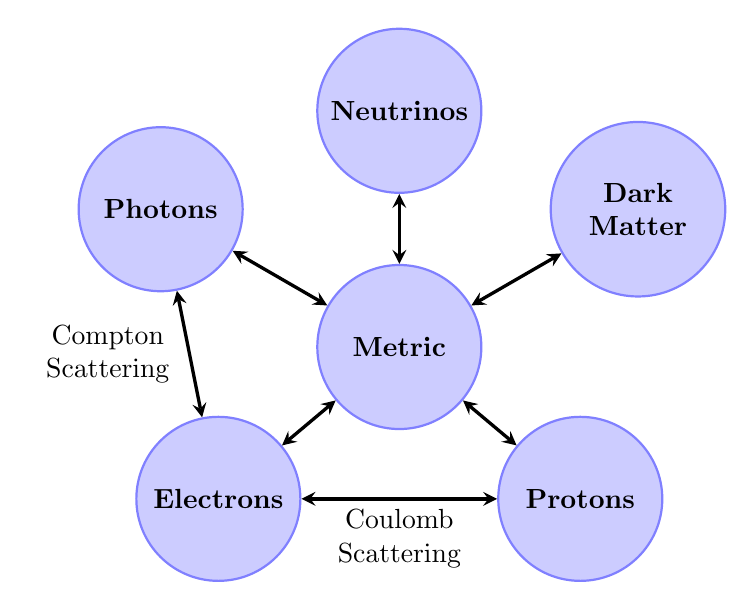
\begin{tikzpicture}[%
    writing/.style={%
      text width=18mm,  % default text width
      align=center      % align in center
    },
    component/.style={%
      circle,           % circular node
      fill=blue!20,     % fill it in blue
      draw=blue!50,     % outside edge in blue
      thick,            %              and thick
      writing,          % writing style above
      font=\bfseries    % bold writing
    },
    connection/.style={%
      <->,             % Double headed
      very thick,      % very thick arrows
      >=stealth        % pretty arrow head
    }
]

    % nodes
    \node at (0,0)     [component] (metric)      {Metric};

    \node at (90 :3)   [component] (neutrinos)   {Neutrinos};
    \node at (150:3.5) [component] (photons)     {Photons};
    \node at (220:3)   [component] (electrons)   {Electrons};    
    \node at (320:3)   [component] (protons)     {Protons};      
    \node at (30 :3.5) [component] (dark matter) {Dark Matter};


    % connections
    \draw[connection] (metric) -- (neutrinos);
    \draw[connection] (metric) -- (photons);
    \draw[connection] (metric) -- (electrons);
    \draw[connection] (metric) -- (protons);
    \draw[connection] (metric) -- (dark matter);

    % interconnections with text
    \draw[connection] 
    (electrons) to 
    node[below,writing] {Coulomb Scattering} 
    (protons);

    \draw[connection] 
    (electrons) to 
    node[left,writing] {Compton Scattering} 
    (photons);

\end{tikzpicture}

%\caption{Composition of the universe, along with the interaction of the components.\label{fig:cos:composition}}
%\end{figure}


\section{Inflation}
The canonical way to explain this early accelerated phase is via the phnomenon of {\em inflation}.


\clearpage{}


%
% Kinetic dominance in the early universe
% ---------------------------------------
%
\makeatletter
\def\input@path{{.}{./chapter_kinetic_dominance/}}
\makeatother
\graphicspath{{.}{./chapter_kinetic_dominance/figures/}}
\chapter{Kinetic Dominance in the early universe}
\label{chap:kd}

\section{Introduction}
\label{sec:kd:intro}

%
% Reconstructing the primordial power spectrum
% --------------------------------------------
%
\makeatletter
\def\input@path{{.}{./chapter_pps_reconstruction/}}
\makeatother
\graphicspath{{.}{./chapter_pps_reconstruction/figures/}}
\chapter{Reconstructing the Primordial Power Spectrum}
\label{chap:rec}

\section{Introduction}
\label{sec:rec:intro}

%
% Defining the quantum vacuum
% ---------------------------
%
\makeatletter
\def\input@path{{.}{./chapter_quantum_vacuum/}}
\makeatother
\graphicspath{{.}{./chapter_quantum_vacuum/figures/}}
\chapter{Defining the Quantum Vacuum}
\label{chap:qv}

\section{Introduction}
\label{sec:qv:intro}

%
% Kinetic initial conditions for inflation
% ----------------------------------------
%
\makeatletter
\def\input@path{{.}{./chapter_kinetic_initial_conditions/}}
\makeatother
\graphicspath{{.}{./chapter_kinetic_initial_conditions/figures/}}
\chapter{Kinetic Initial Conditions for Inflation}
\label{chap:ic}

\section{Introduction}
\label{sec:ic:intro}

%
%
%
%
% Appendices
% ==========
%
\part{Appendices}
%
\appendix
%
\makeatletter
\def\input@path{{.}{./appendix_RKWKB/}}
\makeatother
\graphicspath{{.}{./appendix_RKWKB/figures/}}
\chapter[The RKWKB method]{The Runge-Kutta-Wentzel-Kramers-Brillouin~method}
\label{chp:RK}

\section{Introduction}
\label{sec:introduction}
The numerical solution of linear, ordinary differential equations is of critical importance throughout science and mathematics. In this chapter we suggest an efficient approach for navigating highly oscillatory numerical solutions.

Most traditional numerical solvers of differential equations use a generalisation of Runge-Kutta (RK) techniques \citep{Press+2007}. These apply Taylor's theorem to create a stepping scheme whereby the value of the solution is updated using derivative information. Good solvers will also incorporate adaptive step-size control.
Whilst RK techniques are an excellent workhorse for solving a wide variety of problems, they are known to struggle to solve equations with highly oscillatory solutions.

On the other hand, the Wentzel-Kramers-Brillouin (WKB) method is a well established analytical approach for approximately describing oscillatory solutions \citep{RHB,Bender+2010}. Historically this has been used to approximate the global shape and characteristics of an oscillating solution with a ``slowly changing'' frequency.

We propose that one may combine the two approaches to create a reliable general tool for the numerical solution of oscillatory differential equations, and term the result RKWKB\footnote{Readers with experience in the field will note that, as Cambridge authors, we should be insisting on an additional `J' in WKB (for Jeffreys). Given the length of our proposed acronym, we have opted to use the more efficient nomenclature.}.

We note that this approach is similar to the work of~\cite{Iserles02globalerror,Iserles01thinkglobally}, and explore the similarities and differences in Section~\ref{sec:iserles_comparison}.


\section{Background}
\subsection{Oscillating solutions}
We seek to create a numerical method which efficiently solves linear differential equations such as:
\begin{equation}
  \ddot{x}(t) + {\omega(t)}^2x(t) = 0,\qquad \omega(t)\in\mathbb{R}.
  \label{eqn:lode}
\end{equation}
If \(\omega(t)=\omega = \mathrm{constant}\), then the solutions are sinusoidal: \(x\propto \exp{(\pm i \omega t)}\). If \(\omega(t)\) changes slowly with \(t\), then the solutions are approximately sinusoidal with a slowly varying frequency and amplitude (these ideas will be made more concrete in Section~\ref{sec:wkb}). An example of such a solution can be seen in Figure~\ref{fig:airy}.

In general, any second order linear differential equation may be transformed into the form of~\eqref{eqn:lode} by either changing the independent variable \(t\) or dependent variable \(x\). The method we shall describe can easily be adapted to other linear differential equations, but we shall work with~\eqref{eqn:lode} for its simplicity of exposition.

Equation~\eqref{eqn:lode} is ubiquitous in physics, particularly in quantum mechanics. The authors' particular interest in its efficient solution comes from work in quantum fields in curved spacetime.



Over the next two subsections we will review the traditional techniques available for solving equations such as~\eqref{eqn:lode}.

\begin{figure}[tp]
  \centering
  \includegraphics[width=\textwidth]{chapters/RKWKB/figures/airy}
  \caption{The real and imaginary parts of the function \(\mathrm{Ai}(-t) + \mathrm{Bi(-t)} i\), where \(\mathrm{Ai}\) and \(\mathrm{Bi}\) are the Airy functions of the first and second kind. This is a solution to the equation \({\ddot{x}(t) + t x(t) = 0}\) (equation~\ref{eqn:airy_equation}).}\label{fig:airy}
\end{figure}


\subsection{Runge-Kutta theory}
\label{sec:rk}
We briefly review the theory of numerically solving ordinary differential equations, before discussing why Runge Kutta techniques are an inefficient tool for solving equations such as~\eqref{eqn:lode}.
For a more detailed introduction to the numerical solution of ordinary differential equations we recommend~\cite{Press+2007}.

A general non-linear differential equation in \(n\) variables can be written in terms of vectors as:
\begin{equation}
  \dot{\mathbf{y}}(t) = \mathbf{f}(\mathbf{y}(t),t).
  \label{eqn:ode}
\end{equation}
Note that any higher order differential equation can be re-written in this form by introducing new variables for each of the higher derivative terms.

Runge-Kutta methods work effectively by generalising the Taylor expansion:
\begin{equation}
  \mathbf{y}(t+h)  = \mathbf{y}(t) + h\:\mathbf{f}(\mathbf{y}(t),t) + \mathcal{O}(h^2).
  \label{eqn:euler}
\end{equation}
Given the value of a solution \(\mathbf{y}_j\) at some time \(t_j\), one may advance to the value of the solution \(\mathbf{y}_{j+1}\) at some finite time later \(t_{j+1} = t_j + h\) by using the recursion relation:
\begin{align}
  \mathbf{y}_{j+1} &=  \mathbf{y}_{j} + h\:\mathbf{f}(\mathbf{y}_j,t_j),
  \label{eqn:y_step}\\
  t_{j+1} &=  t_{j} + h.
  \label{eqn:t_step}
\end{align}
This is termed {\em Euler's method}, and for arbitrarily small \(h\) will recover the solution to any desired accuracy. It is termed {\em first order\/} since each step is accurate to \(\bigO{h}\).

Euler's method is normally impractical for real numerical work. Runge-Kutta schemes work by generalising~\eqref{eqn:euler}~\&~\eqref{eqn:y_step} by including additional intermediate function evaluations that integrate~\eqref{eqn:ode} with greater accuracy.

A possibly more important adjustment is to equip the algorithm with the ability to choose the step size \(h\) according to the accuracy required. A popular stratagem is to run two steps, one of order \(p\), and another of order \(p-1\), and use the difference between the two as an estimate of the error. Particularly smart algorithms use the same function evaluations for both orders. An example of this is the Runge-Kutta-Fehlberg \(4(5)\) method detailed in Section~\ref{sec:rkf}.

All methods based on this principle struggle to solve equations such as~\eqref{eqn:lode} when the algorithm must scale a very large number of peaks and troughs. Errors accumulate rapidly in these approaches, even if the variation of \(\omega(t)\) in \(t\) is very simple. Given the regularity of the solution from Figure~\ref{fig:airy}, one would imagine that there should be a more efficient method.


\subsection{WKB theory}
\label{sec:wkb}
WKB approaches are designed to solve linear ordinary differential equations like~\eqref{eqn:lode} in the limit of a ``slowly varying'' \(\omega(t)\): i.e.\ the fractional change in frequency \(\frac{\Delta\omega}{\omega}\) over several time periods \(\Delta t \sim \frac{2\pi}{\omega}\) is relatively small.
A systematic way of phrasing this is to rescale the independent variable of~\eqref{eqn:lode} so \(t\rightarrow t/T\):
\begin{equation}
  \ddot{x}(t) + T^{-2}{\omega(t)}^2x(t) = 0,\qquad \omega(t)\in\mathbb{R}.
  \label{eqn:lode_T}
\end{equation}
If \(T\gg1\) then \(\omega\) is slowly varying, or equivalently the solutions have very rapid oscillations (large \(\omega\)). Given this, one can expand the solutions in terms of complex exponential functions:
\begin{equation}
  x(t)\sim \exp\left( \frac{1}{T}\sum\limits_{n=0}^{\infty} S_n(t)\: T^n \right).
  \label{eqn:asymp}
\end{equation}
Substituting this into~\eqref{eqn:lode_T} and setting each coefficient of \(T\) equal to zero yields a sequence of solvable equations. One finds the first four solutions are:
\begin{align}
  S_0(t) &= \pm i \int^t \omega(\tau)\: \d{\tau},
  \label{eqn:S0}\\
  S_1(t) &= -\frac{1}{2}\log \omega(t),\\
  S_2(t) &=  \mp i \int^t \frac{1}{4}\frac{\ddot{\omega}(\tau)}{\omega^{2}(\tau)} - \frac{3}{8}\frac{\dot{\omega}^2(\tau)}{\omega^{3}(\tau)}\: \d{\tau}, \\
  S_3(t) &=  \frac{1}{8}\frac{\ddot{\omega}(t)}{\omega^{3}(t)} - \frac{3}{16} \frac{\dot{\omega}^{2}(t)}{\omega^{4}(t)}.
\end{align}
and in general:
\begin{equation}
    \dot{S}_0(t) = \pm i \omega, \qquad \dot{S}_n = -\frac{1}{\dot{S}_0} \left( \ddot{S}_{n-1}+ \sum_{j=1}^{n-1}\dot{S}_j\dot{S}_{n-j}  \right)
\end{equation}
Note that at \(0\)\textsuperscript{th} order, the solution is \(x\propto\exp\left(\pm i \int \omega \d{t} \right)\), which should be compared with the traditional sinusoidal solution.
Typically \(T\) is considered a power counting parameter, and set equal to \(1\) at the end of the analysis.

There are two integration constants associated with the either sign of equation~\eqref{eqn:S0}. The other integration constants from the remaining equations may be absorbed into the first two. The \(n\)\textsuperscript{th} order solution thus takes the form:
\begin{align}       
  x_\mathrm{WKB}^{(n)}[A_{\pm}](t) &=
  A_{+} e^{\phi_+(t)} + A_{-} e^{\phi_-(t)},
  \label{eqn:solution} \\
  \phi_\pm(t) &= \sum_{i=0}^{n} S_i(t).
  \label{eqn:phidef} 
\end{align}
If one has initial conditions at time \(t_0\):
\begin{equation}
  x(t_0) = x_0, \qquad \dot{x}(t_0)=\dot{x}_0,
  \label{eqn:i_c}
\end{equation}
then the coefficients \(A_\pm\) may be determined by:
\begin{equation}
    A_\pm(x_0,\dot{x}_0,t_0) = \frac{x_0 \dot{\phi}_\mp- \dot{x}_0 }{\dot{\phi}_\mp - \dot{\phi}_\pm} e^{-\phi_\pm},
  \label{eqn:i_c_Apm}
\end{equation}
where all \(\phi\) variables are evaluated at \(t_0\).
We can perform the same analysis with the derivative of~\eqref{eqn:asymp}:
\begin{equation}       
  \dot{x}_\mathrm{WKB}^{(n)}[B_{\pm}](t) =
  B_{+} \dot{\phi}_+(t)e^{\phi_+(t)} + B_{-} \dot{\phi}_-(t)e^{\phi_-(t)}.
  \label{eqn:solution_xdot}
\end{equation}
If one has initial conditions at time \(t_0\):
\begin{equation}
  \dot{x}(t_0) = \dot{x}_0, \qquad \ddot{x}(t_0)=\ddot{x}_0,
  \label{eqn:i_c_xdot}
\end{equation}
then the coefficients \(B_\pm\) may be determined by:
\begin{equation}
    B_\pm(\dot{x}_0,\ddot{x}_0,t_0) = \frac{\dot{x}_0(\ddot{\phi}_\mp+\dot{\phi}_\mp^{2})-\ddot{x}_0\dot{\phi}_\mp}{\dot{\phi}_\mp^{2}\dot{\phi}_\pm-\dot{\phi}_\pm^{2}\dot{\phi}_\mp+\ddot{\phi}_\mp\dot{\phi}_\pm-\ddot{\phi}_\pm\dot{\phi}_\mp} {{e}^{-{\phi}_\pm}},
  \label{eqn:i_c_Bpm}
\end{equation}
where all \(\phi\) variables are evaluated at \(t_0\).
For further detail on the intricacies of WKB approaches, the reader should 

\section{The RKWKB method}
Our strategy is to combine the versatility of RK methods with the power of WKB in dealing with oscillating solutions. We term the combination RKWKB\@.

Given a function \(\omega(t)\), one proposes a step in time of \(h\) to be accompanied by an updating of the solution \(x_j\) via:
\begin{align}
  x_{j+1} &= x_\mathrm{WKB}^{(n)}[A_\pm(x_j,\dot{x}_j,t_j)](t_j+h),
  \label{eqn:WKB_x_step} \\
  \dot{x}_{j+1} &= \dot{x}_\mathrm{WKB}^{(n)}[B_\pm(\dot{x}_j,\ddot{x}_j,t_j)](t_j+h),
  \label{eqn:WKB_xdot_step} \\
  t_{j+1} &= t_j+h,
  \label{eqn:WKB_t_step} \\
  \ddot{x}_{j+1} &= -\omega^2(t_{j+1})x_{j+1},
  \label{eqn:WKB_xddot} 
\end{align}
where \(x_\mathrm{WKB}^{(n)}[A_{\pm}]\) and \(\dot{x}_\mathrm{WKB}^{(n)}[B_{\pm}]\) are given by~\eqref{eqn:solution} and~\eqref{eqn:solution_xdot},  and \(A_{\pm}\) and \(B_{\pm}\)  are given by~\eqref{eqn:i_c_Apm} and~\eqref{eqn:i_c_Bpm}.

To paraphrase the above; one matches the \(n\)\textsuperscript{th} order WKB solution onto the current values of \(x_j\) and \(\dot{x}_j\), and uses this to extrapolate the solution by a time step of \(h\). We repeat the same process for the derivative \(\dot{x}_j\), using its own WKB expansion. Finally, we self-consistently fix \(\ddot{x}_j\) so that it satisfies equation~\eqref{eqn:lode}. Since WKB naturally encodes the oscillatory nature of the solution, this will allow step sizes \(h\) to be far larger than a single period of oscillation. 

%Note the importance of using two WKB expansions with coefficients \(A_\pm\) and \(B_\pm\) to step \(x_j\) and \(\dot{x}_j\) separately. If we used the same coefficients to step both, then one would simply be following the same WKB solution.

\subsection{To be moved: General expansion methods}
In the general case, one aims to solve a linear, second order differential equation in \(x(t)\) whereby one has two analytical linearly independent approximate solutions \(f_\pm(t)\), as well as access to their derivatives \(\dot{f}_\pm\) and \(\ddot{f}_\pm\). At a given time \(t_j\) with values of the true solution \(x_j\) and its derivative \(\dot{x}_j\), one may match the approximate solutions onto the correct solution:
\begin{align}
    x(t) &\approx  A_+ f_+(t) + A_- f_-(t) \\
    A_\pm &= \frac{\dot{x}_j f_\mp(t_j) - x_j \dot{f}_\mp(t_j) }{\dot{f}_\pm(t_j) f_\mp(t_j) - \dot{f}_\mp(t_j) f_\pm(t_j)}.
\end{align}
This has the property of providing an excellent approximation to the true solution in the region \(t=t_j + h\) where \(h\) is small. The degree of its failure is then determined by how well the solutions \(f_\pm\) trace the true solutions. 
One may perform the same operation above for its derivative
\begin{align}
    \dot{x}(t) &\approx  B_+ \dot{f}_+(t) + B_- \dot{f}_-(t) \\
    B_\pm &= \frac{\ddot{x}_j \dot{f}_\mp(t_j) - \dot{x}_j \ddot{f}_\mp(t_j) }{\ddot{f}_\pm(t_j) \dot{f}_\mp(t_j) - \ddot{f}_\mp(t_j) \ddot{f}_\pm(t_j)}, 
\end{align}
noting that in the second order case, one may determine \(\ddot{x}\) from \(\dot{x}\) and \(x\) via the original second order linear differential equation.

The general stepping procedure is then as follows:
\begin{align}
  x_{j+1} &= A_+ f_+(t_j + h) + A_- f_-(t_j + h)
  \label{eqn:x_step} \\
  \dot{x}_{j+1} &= B_+ \dot{f}_+(t_j + h) + B_- \dot{f}_-(t_j + h)
  \label{eqn:x_dot_step} \\
  t_{j+1} &= t_j+h,
  \label{eqn:t_step}
\end{align}
and at every iteration \(t_j\), \(\ddot{x}_j\) is determined from \(\dot{x}_j\) and \(x_j\) via the original second order linear differential equation.

\subsection{The necessity of two expansions}
It is not immediately obvious why we require separate expansions for \(x\) and \(\dot{x}\) in the method detailed above, utilising four coefficients \(A_\pm\) and \(B_\pm\). Indeed, an early version of this algorithm simply used a single WKB expansion as a stepper for both \(x\) and \(\dot{x}\): 
\begin{align}
  x_{j+1} &= A_+ f_+(t_j + h) + A_- f_-(t_j + h) \tag{WRONG!},\\
  \dot{x}_{j+1} &= A_+ \dot{f}_+(t_j + h) + A_- \dot{f}_-(t_j + h) \tag{WRONG!},\\
  t_{j+1} &= t_j+h \tag{WRONG!}
\end{align}
Alas, such a method is doomed to failure\footnote{Credit here is due to Prof.\ Anthony Challinor for spotting our error.}. Simply put, since a given solution is defined entirely by the value of \(x\) and \(\dot{x}\) at a single point, using the values \(x_j\) and \(\dot{x}_{j}\) to forecast onto \(x_{j+1}\) and \(\dot{x}_{j+1}\) merely replicates the solution of the previous step.  The method then merely follows a single curve ad infinitum.

One can see this more concretely by observing that this method should replicate a simple Runge-Kutta approach in the limit of vanishing step size \(h\). The single stepper does not. In the limit of small \(h\), one has:
\begin{align}
    f(t_{j+1}) &\approx f(t_j) + \dot{f}(t_j) \: h +\mathcal{O}(h^2),  \tag{WRONG!} \\
    \dot{f}(t_{j+1}) &\approx f(t_j) + \ddot{f}(t_j) \: h +\mathcal{O}(h^2), \tag{WRONG!} \\
    \Rightarrow x_{j+1} &= x_j + \dot{x}_j \: h , \tag{WRONG!} \\
    \Rightarrow \dot{x}_{j+1} &= \dot{x}_j + 
    \frac{(\ddot{f}_+ f_- - \ddot{f}_- f_+)\dot{x}_j  +( \ddot{f}_- \dot{f}_+- \ddot{f}_+ \dot{f}_-)x_j}{\dot{f}_+ f_- - \dot{f}_- f_+}\: h
    , \tag{WRONG!}
\end{align}
where in the final equation, all \(f\) terms are evaluated at \(t_j\).

If however, we use two expansions, then by definition (or rather laborious algebra):
\begin{align}
    x_{j+1} &= x_j + \dot{x}_j \: h, \\
    \dot{x}_{j+1} &= \dot{x}_j + \ddot{x}_j \: h.
\end{align}



\subsection{Step size adjustment}
To tune the step size \(h\), we use the same strategy as adaptive Runge-Kutta schemes. We compute both the order \(n\) and order \(n-1\) WKB solutions, and use the fractional difference between the two:
\begin{equation}
  \varepsilon = \left|\frac{x^{(n)}-x^{(n-1)}}{x^{(n)}}\right|,
  \nonumber
\end{equation}
as an estimate of the truncation error. 

We now assume that the desired accuracy is \(\alpha\). If \(\varepsilon<\alpha\) then the solution is within the desired tolerance, and the algorithm makes a step of size \(h\). \(h\) is then increased for the next iteration. If \(\varepsilon>\alpha\) then the step is unsuccessful, and the step size is reduced. \(h\) may therefore be efficiently updated between attempts via:
\begin{equation}
  h \to h\times\left\{
  \begin{array}{lr}
    {(\alpha/\varepsilon)}^{1/n} &: \varepsilon<\alpha \\
    {(\alpha/\varepsilon)}^{1/(n-1)} &: \varepsilon>\alpha. \\
  \end{array}
  \right.\label{eqn:h_update}
\end{equation}
This allows the step size to increase in the regions where the initial step size is unnecessarily small, whilst ensuring that the step size is always small enough to keep forecasts within a given error margin.

\subsection{Dynamic switching}
In general, one cannot expect the WKB expansion to be efficient throughout the solution region. If \(\omega\) is too small, or too quickly varying, then the step size \(h\) will decrease to an inefficiently small size. This problem can be countered by simultaneously attempting a step using a standard adaptive RK method. One chooses between RK and WKB by selecting the method with the smallest error. This provides a natural switching mechanism, without having to delve into the details of whether WKB is valid or not.

We choose the Runge-Kutta-Fehlberg \(4(5)\) method for our alternative solver, which is detailed in Section~\ref{sec:rkf}. However, this may be substituted with any ODE solver according to the user's preference.

\section{Example: The Airy equation}


As an example of the RKWKB approach, we apply it to the Airy equation:
\begin{align}
  0=\ddot{x}(t) &+ t\: x(t) ,
  \label{eqn:airy_equation}\\
  x(0)=\frac{3^{-2/3}+3^{-1/6}i}{\Gamma(2/3)},
  &\qquad
  \dot{x}(0) = \frac{3^{-1/3}-3^{1/6}i}{\Gamma(1/3)},
  \nonumber\\
  \Rightarrow x(t) = \mathrm{Ai}(-t) &+ \mathrm{Bi}(-t)\:i,
  \label{eqn:airy_solution}
\end{align}
whose solution is depicted in Figure~\ref{fig:airy}. This is often quoted as being a ``maximally hard'' problem for RK machinery to solve, since the frequency steadily increases, causing the step size to get smaller as the algorithm goes deeper into the solution.

We set the desired relative error to be \(10^{-4}\). The algorithm remains in the RK regime until \(t\sim5\). When the WKB solver is activated, instead of following every oscillation of the solution, it rapidly speeds up, skipping many oscillations. This is detailed in Figure~\ref{fig:data}.

The error compared to the true solution is detailed in Figure~\ref{fig:error}. Here we find that initially the error is small, but grows\(\bigO{h^{2s} t^{s+5/4}}\) where \(s=4\) is the order of the RK method \citep{Iserles02globalerror}. After the WKB regime is entered, it begins to make huge strides, and the error levels off.

In contrast to a ``pure'' RK method, the RKWKB method finds the Airy equation maximally {\em easy}.



\begin{figure}[tp]
  \centering
  \includegraphics[width=\textwidth]{chapters/RKWKB/figures/data}
  \caption{The RKWKB method compared with the analytical solution. The algorithm starts at \(t=0\) in the RK regime, since \(\omega\) is varying quickly relative to the oscillation period. At \(t=5\) it becomes more efficient to use the WKB regime, and the points start to increase in separation. By \(t=15\) the algorithm is skipping multiple periods, and the step size \(h\) increases exponentially.}\label{fig:data}
\end{figure}

\begin{figure}[tp]
  \centering
  \includegraphics[width=\textwidth]{chapters/RKWKB/figures/error}
  \caption{Fractional difference between the analytical solution and RKWKB solution from Figure~\protect\ref{fig:data}. The algorithm's fractional error begins at \(t=0\) with an error of \(\sim10^{-4}\), but rises in the RK phase. This is to be expected as RK methods accumulate errors (particularly for oscillatory solutions). Upon entering the WKB region, the fractional error levels off. Note the rapidly increasing step size, and accuracy at extremely late times \(t\). To the authors' knowledge, no numerical scheme to date has demonstrated the ability to solve the Airy equation~\protect\eqref{eqn:airy_equation} to times as late as this.}\label{fig:error}
\end{figure}




\section{Comparison with the Iserles approach}
\label{sec:iserles_comparison}
Iserles has written extensively on the difficulty of solving problems of the form~\eqref{eqn:lode}. His approach is to turn~\eqref{eqn:lode} into a Lie-group differential equation \citep{Iserles00lie-groupmethods} by writing:
\begin{align}
  \mathbf{y} &= {(x,\dot{x})}^\top, 
  \mathrm{A}(t) = 
  \left(
  \begin{array}{cc}
    0 & 1 \\
    -\omega^2(t) & 0
  \end{array}
  \right),
  \nonumber\\
  \Rightarrow\quad 
  \dot{\mathbf{y}} &= \mathrm{A} (t) \: \mathbf{y}.\label{eqn:lie_eqn}
\end{align}
This may then be attacked with a variety of Lie group methods. For example, one may write the full solution as a Magnus expansion:
\begin{align}
  \mathbf{x}(t) &= e^{\Omega(t,t_0)} \mathbf{x}_0,
  \label{eqn:magnus}\\
  \Omega(t,t_0) &= \int_{t_0}^t \mathrm{A}(x) \d{x} \nonumber \\
  &- \frac{1}{2}\int_{t_0}^t\int_{t_0}^{x_1} \left[\mathrm{A}(x_2),\mathrm{A}(x_1)\right] \d{x_2} \d{x_1} + \ldots
  \nonumber
\end{align}
and then use a truncated series to create a stepping algorithm.
This approach is much improved by transferring to a fast rotating frame:
\begin{equation}
  \mathbf{y}(t_n+\tau) = e^{\tau \mathrm{A}(t_n+h/2)} \mathbf{x},
  \label{eqn:rotating_frame}
\end{equation}
the end product is then termed the {\em modified Magnus method\/} \citep{Iserles01thinkglobally}.

The RKWKB method and the modified Magnus method share some key features. Indeed, the lowest order modified Magnus method is equivalent to a \(1\)\textsuperscript{st} order WKB approach \citep{Iserles02globalerror}. However, our approach is distinguished in several ways. 

First, the Magnus expansion~\eqref{eqn:magnus} requires multiple integrals for higher order terms. These integrals are tricky to implement, and can introduce considerable computational overhead. The WKB expansion~\eqref{eqn:WKB_x_step} on the other hand requires at most single integrals, replacing the double integrals with additional derivative terms of \(\omega\), which are typically easier to compute.

Second, our approach uses adaptive step-size control, which is very easy to implement in the WKB framework and crucial for real-world numerical work.

Finally, by using dynamic switching, the algorithm is able to utilise the optimal approach in real time.

However, Iserles' approach has been the inspiration for this work, and we believe that many of the difficulties associated with the implementation of Magnus methods are merely engineering problems. We believe that in the fullness of time Magnus methods could become the de-facto numerical integration tool. In the mean-time, this work provides a simpler, more streamlined methodology.


\section{Conclusions}



We have presented a novel method for numerically solving linear differential equations with highly oscillatory solutions. We use a Wentzel-Kramers-Brillouin expansion to create an adaptively stepping algorithm in the same manner as a Runge-Kutta scheme. Further, the algorithm will switch back to a normal RK approach when the frequency of oscillation is varying too quickly for WKB to approximate accurately. The method is compared to Iserles existing approaches, and found to be a reasonable alternative without requiring the use of heavy Lie-group machinery. This chapter is not intended to be a complete exposition, but more a proof-of-principle to create a springboard for further investigation.



\begin{subappendices}
  \section{Runge-Kutta-Fehlberg}
\label{sec:rkf}

A general explicit RK method can be written as:
\begin{align}
  y_{n+1} &= y_n + h\sum\limits_{i=1}^{s} b_i k_i, \label{eqn:rk_step} \\
  k_s &= f(t_n + c_s h, y_n + h \sum\limits_{i=1}^{s-1}a_{si} k_i),
\end{align}
where the coefficients $\{c_i,a_{si}\}$ are determined by the choice of method and are typically written in a Butcher tableau (Table~\ref{tab:RKexplicit}). 

A particularly efficient example is the Runge-Kutta-Fehlberg $4(5)$ method which uses an embedded approach. It performs a fourth order step and a fifth order step, and uses the difference between these as an estimate of the error. Impressively, both steps are calculated using the same values of $\{k_i\}$ (but different values of $\{b_i\}$), and hence the method only requires five function evaluations of $f$ per step. Its Butcher tableau is detailed in Table~\ref{tab:rkf45}.

\begin{table}[h]
  \begin{equation*}
    \begin{array}{l | c c c c c}
      0      \quad &               &              &              &         &   \\
      c_2    \quad & \quad a_{21}  &              &              &         &   \\
      c_3    \quad & \quad a_{31}  & \quad a_{32} &              &         &   \\
      \vdots \quad & \quad \vdots  & \quad \vdots & \quad \ddots &         &   \\
      c_s    \quad & \quad a_{s1}  & \quad a_{s2} & \quad \cdots & \quad a_{s,s-1} & \\ \midrule
      & \quad b_{1}   & \quad b_{2}  & \quad \cdots & \quad b_{s-1}  & \quad b_{s}
    \end{array}
  \end{equation*}
  \caption{Butcher tableau for a general explicit RK method.\label{tab:RKexplicit}
  }
\end{table}

\begin{table}
  \begin{equation*}
    \begin{array}{l | c c c c c c}
      0      &           &            &             &             &        &\\
      \frac{1}{4}    & \frac{1}{4}       &            &             &             &        &\\
      \frac{3}{8}    & \frac{3}{32}      & \frac{9}{32}       &             &             &        &\\
      \frac{12}{13}  & \frac{1932}{2197} & -\frac{7200}{2197} & \frac{7296}{2197}   &             &        &\\
      1      & \frac{439}{216}   & -8         & \frac{3680}{513}    & -\frac{845}{4104}   &        &\\
      \frac{1}{2}    & -\frac{8}{27}     & 2          & -\frac{3544}{2565}  & \frac{1859}{4104}   & -\frac{11}{40} &\\\midrule
      & \frac{25}{216}    & 0          & \frac{1408}{2565}   & \frac{2197}{4104}   & -\frac{1}{5}   & 0      \\
      & \frac{16}{135}    & 0          & \frac{6656}{12825}  & \frac{28561}{56430} & -\frac{9}{50}  & \frac{2}{55}
    \end{array}
  \end{equation*}
  \caption{Butcher tableau for the embedded Runge-Kutta-Fehlberg $4(5)$ method.\label{tab:rkf45}                                                             }
\end{table}




\end{subappendices}


%
% The bibliography
%
% Basic bibliography style
\bibliographystyle{plainnat}

% BibTex bibliography
\bibliography{other/references}


%
\end{document}

